%\documentclass{article}
\documentclass[10pt,a4paper]{article}

% Optional: Better font and spacing
\usepackage{libertine} % Libertine font
\usepackage{microtype}


\usepackage[utf8]{inputenc}

\title{Solutions - Christian Thierfelder}
%\autor{}
%\date{}


%MATH
\usepackage{amsmath}
\usepackage{amsfonts}
\usepackage{amsthm}
\usepackage{amsbsy}
\usepackage{cancel}
\usepackage{relsize}

\usepackage{algorithm}
\usepackage{algorithmic}

\usepackage{units}
\usepackage{mathrsfs}
\usepackage{slashed}
\usepackage{mathtools} %\mathclap - underbrace

\usepackage{hyperref}
\usepackage{simplewick}


\newtheorem{remark}{Remark}[section]
\theoremstyle{definition}
\newtheorem{definition}{Definition}[section]
\newtheorem{theorem}{Theorem}[section]

\DeclareMathOperator{\Aut}{Aut}
\DeclareMathOperator{\GL}{GL}

%PAGELAYOUT
\usepackage{a4wide}

%GRAPHICS
\usepackage{graphicx}
\usepackage[dvipsnames]{xcolor}
\usepackage{tikz}
\usepackage[outline]{contour} % glow around text
\usepackage{xfrac}

\usetikzlibrary{shapes}
\usetikzlibrary{snakes}
\usetikzlibrary{plotmarks}
\usetikzlibrary{decorations.markings}

\usepackage{pgfplots}
\usepgfplotslibrary{polar}

%HYPERLINKS
\usepackage{hyperref}
\hypersetup{
    colorlinks=true,
    linkcolor=blue,
    filecolor=magenta,      
    urlcolor=cyan,
}

\usepackage[shortlabels]{enumitem}

\usepackage{etoolbox}
\providetoggle{includeCoverPic}
\settoggle{includeCoverPic}{true}
%\settoggle{includeCoverPic}{false}
\usepackage{subfiles}

\tikzset{>=latex} % for LaTeX arrow head
\colorlet{myred}{red!85!black}
\colorlet{mydarkred}{red!55!black}
\colorlet{mylightred}{red!85!black!12}
\colorlet{myfieldred}{mydarkred!5} % for S' background
\colorlet{myredhighlight}{myred!20} % highlights simultaneity in ladder paradox
\colorlet{myblue}{blue!80!black}
\colorlet{mydarkblue}{blue!50!black}
\colorlet{mylightblue}{blue!50!black!30}
\colorlet{mylightblue2}{myblue!10}
\colorlet{mygreen}{green!80!black}
\colorlet{mypurple}{blue!40!red!80!black}
\colorlet{mydarkgreen}{green!50!black}
\colorlet{mydarkpurple}{blue!40!red!50!black}
\colorlet{myorange}{orange!40!yellow!95!black}
\colorlet{mydarkorange}{orange!40!yellow!85!black}
\colorlet{mybrown}{brown!20!orange!90!black}
\colorlet{mydarkbrown}{brown!20!orange!55!black}
\colorlet{mypurplehighlight}{mydarkpurple!20} % highlights simultaneity in ladder paradox
\tikzstyle{world line}=[myblue!40,line width=0.3]
\tikzstyle{world line t}=[mypurple!50!myblue!40,line width=0.3]
\tikzstyle{world line'}=[mydarkred!40,line width=0.3]
\tikzstyle{mysmallarr}=[-{Latex[length=3,width=2]},thin]
\tikzstyle{mydashed}=[dash pattern=on 3 off 3]
\def\Nsamples{100}
\tikzstyle{vector}=[->,line width=1,line cap=round]
\tikzstyle{vector'}=[vector,shorten >=1.2]
\tikzstyle{particle}=[mygreen,line width=0.9]


\usepackage{geometry}
\geometry{
  a4paper,
  left=1.5cm,
  right=2cm,
  top=2cm,
  bottom=2cm
}

\newcommand{\feynPropagator}{
  \raisebox{0.2em}{%
    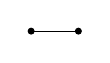
\begin{tikzpicture}[scale=0.3, baseline]
    \coordinate (A) at (-1,0);
      \coordinate (B) at (1,0);
      \draw (A) -- (B);
	  \filldraw (A) circle (3.5pt);
      \filldraw (B) circle (3.5pt);
    \end{tikzpicture}%
  }
}

\newcommand{\feynOneLoop}{
  \raisebox{0.2em}{%
    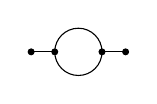
\begin{tikzpicture}[scale=0.3, baseline]
      \coordinate (A) at (-2,0);
      \coordinate (B) at (-1,0);
      \coordinate (C) at (1,0);
      \coordinate (D) at (2,0);
      \draw (A) -- (B);
      \draw (0,0) circle (1.0);
      \draw (C) -- (D);
	  \filldraw (A) circle (3.5pt);
      \filldraw (B) circle (3.5pt);
      \filldraw (C) circle (3.5pt);
      \filldraw (D) circle (3.5pt);
    \end{tikzpicture}%
  }
}

\newcommand{\feynBaloon}{
  \raisebox{-1.0em}{%
    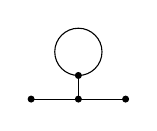
\begin{tikzpicture}[scale=0.3, baseline]
      \coordinate (A) at (-2,0);
      \coordinate (B) at (0,0);
      \coordinate (C) at (0,1);
      \coordinate (D) at (2,0);
      \draw (A) -- (B);
      \draw (B) -- (C);
      \draw (B) -- (D);
      \draw (0,2) circle (1.0);
	  \filldraw (A) circle (3.5pt);
      \filldraw (B) circle (3.5pt);
      \filldraw (C) circle (3.5pt);
      \filldraw (D) circle (3.5pt);
    \end{tikzpicture}%
  }
}


\newcommand{\feynTwoDisconn}{
  \raisebox{0.2em}{%
    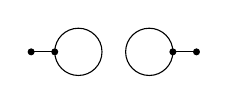
\begin{tikzpicture}[scale=0.3, baseline]
      \coordinate (A) at (-2,0);
      \coordinate (B) at (-1,0);
      \coordinate (C) at (4,0);
      \coordinate (D) at (5,0);
      \draw (A) -- (B);
      \draw (0,0) circle (1.0);
      \draw (3,0) circle (1.0);
      \draw (C) -- (D);
	  \filldraw (A) circle (3.5pt);
      \filldraw (B) circle (3.5pt);
      \filldraw (C) circle (3.5pt);
      \filldraw (D) circle (3.5pt);
    \end{tikzpicture}%
  }
}

\newcommand{\feynTwoLoops}{
  \raisebox{0.2em}{%
    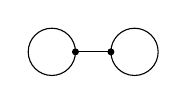
\begin{tikzpicture}[scale=0.3, baseline]
      \coordinate (A) at (-1,0);
      \coordinate (B) at (+0.5,0);
      \draw (-2,0) circle (1.0);
      \draw (A) -- (B);
      \draw (+1.5,0) circle (1.0);
	  \filldraw (A) circle (3.5pt);
      \filldraw (B) circle (3.5pt);
    \end{tikzpicture}%
  }
}

\newcommand{\feynOneLoopConnect}{
  \raisebox{0.2em}{%
    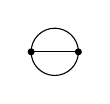
\begin{tikzpicture}[scale=0.3, baseline]

      \coordinate (B) at (-1,0);
      \coordinate (C) at (1,0);
      \draw (B) -- (C);
      \draw (0,0) circle (1.0);
      \filldraw (B) circle (3.5pt);
      \filldraw (C) circle (3.5pt);
    \end{tikzpicture}%
  }
}





\begin{document}

\centerline{{\Large Solutions - Christian Thierfelder}}
%\maketitle




\section{Quantum Field Theory II – Exercise sheet 1 2025-04-29}
\subsection{Exercise 1 - Two-point function in interacting QFT}
{\color{blue} Consider $\phi^3$ theory with action
\begin{align}
S=\frac{1}{2}\int d^4x\;\phi(x)\left[m^2-\Box\right]\phi(x)-\frac{\lambda}{3!}\int d^4x\;\phi^3(x) \tag{1}
\end{align}

\begin{enumerate}[1.]
\item Compute the two-point functions $\langle\phi(x_1)\phi(x_2)\rangle$ to second order in perturbation theory (to order $\lambda^2$) by use of the Gell-Mann-Low formula.
\item Compute the two-point functions $\langle\phi(x_1)\phi(x_2)\rangle$ to order $\lambda^2$ by use of the Schwinger-Dyson equations.
\end{enumerate}
}

\begin{enumerate}[1.]
\item Gell-Man-Low formula
\begin{align}
\mathcal{L}_{int}&=-\frac{\lambda}{3!}\int d^4x\,\phi^3(x)\\
\mathcal{H}_{int}&=+\frac{\lambda}{3!}\int d^4x\,\phi^3(x)\\
\langle\phi(x_1)\phi(x_2)\rangle
&=\frac{\langle0| T\{\phi(x_1)\phi(x_2)\exp(-i\int d^4x\mathcal{H}_{int})\}|0\rangle}{\langle0| T\{\exp(-i\int d^4x\mathcal{H}_{int})\}|0\rangle}\\
&=\frac{\langle0| T\{\phi(x_1)\phi(x_2)\exp(-i\frac{\lambda}{3!}\int d^4x\,\phi^3(x))\}|0\rangle}{\langle0| T\{\exp(-i\frac{\lambda}{3!}\int d^4x\,\phi^3(x))\}|0\rangle}
\end{align}
Using Wicks theorem we see that due to the $\phi^3$ interaction the first orders of numerator (power: $2+3=5$) and denominator (power: 3) vanish.
\begin{itemize}
\item Denominator
\begin{align}
\langle0| T\{&\exp\left(-i\frac{\lambda}{3!}\int d^4x\,\phi^3(x)\right)\}|0\rangle\\
&\simeq\langle0| T\{\left(1-i\frac{\lambda}{3!}\int d^4x\,\phi^3(x)+\frac{i^2}{2}\frac{\lambda^2}{(3!)^2}\iint d^4xd^4y\,\phi^3(x)\phi^3(y)\right)\}|0\rangle\\
&\simeq\langle0| 0\rangle
-i\frac{\lambda}{3!}\int d^4x\, \cancel{\langle0|\phi^3(x)|0\rangle}
-\frac{\lambda^2}{2(3!)^2}\iint d^4xd^4y\, \langle0| T\{\phi^3(x)\phi^3(y)\}|0\rangle\\
&\simeq 1 - \frac{\lambda^2}{2(3!)^2}\cdot \left[\;6\times\feynOneLoopConnect,\;9\times\feynTwoLoops\;\right]\\
&\simeq 1 - \frac{\lambda^2}{2(3!)^2}\iint d^4x\,d^4y \left[6\cdot(\Delta_F(x-y))^3+9\cdot(\Delta_F(0))^2\Delta_F(x-y)\right]
\end{align}
\begin{itemize}
\item Each $\phi(x)$ contracts with a $\phi(y)$: $3\cdot2\cdot1=6\;\times\;\Delta_F(x-y)$
\item Two $\phi(x)$ and two $\phi(y)$ contract and the remaining $\phi(x)$ contracts with $\phi(y)$: $3\cdot3=9 \times (\Delta_F(0))^2\Delta_F(x-y)$
\item Double check combination count: $(6-1)!!=\frac{6!}{2^{6/2}\cdot3!}=15=6+9$
\end{itemize}
\item Numerator
\begin{align}
\langle0&| T\{\phi(x_1)\phi(x_2)\exp\left(-i\frac{\lambda}{3!}\int d^4x\,\phi^3(x)\right)\}|0\rangle\\
&\simeq\langle0| T\{\phi(x_1)\phi(x_2)\left(1-i\frac{\lambda}{3!}\int d^4x\,\phi^3(x)+\frac{i^2}{2}\frac{\lambda^2}{(3!)^2}\iint d^4xd^4y\,\phi^3(x)\phi^3(y)\right)\}|0\rangle\\
&\simeq\langle0| T\{\phi(x_1)\phi(x_2)\}|0\rangle
-i\frac{\lambda}{3!}\int d^4x\, \cancel{\langle0|T\{\phi(x_1)\phi(x_2)\phi^3(x)\}|0\rangle}\\
&\qquad-\frac{\lambda^2}{2(3!)^2}\iint d^4xd^4y\, \langle0| T\{\phi(x_1)\phi(x_2)\phi^3(x)\phi^3(y)\}|0\rangle
\end{align}
\begin{align}
\langle0&| T\{\phi(x_1)\phi(x_2)\exp\left(-i\frac{\lambda}{3!}\int d^4x\,\phi^3(x)\right)\}|0\rangle\\
&\simeq 1\cdot\left[\;\feynPropagator\;\right] - \frac{\lambda^2}{2(3!)^2}\cdot \left[\;36\times\feynOneLoop,\,36\times\feynBaloon,\;18\times\feynTwoDisconn,\,6\times\feynPropagator\;\feynOneLoopConnect,\right.\\
&\qquad\qquad\qquad\left.\,9\times\feynPropagator\;\feynTwoLoops\right]\\
&\simeq \Delta_F(x_1-x_2) - \frac{\lambda^2}{2(3!)^2}\iint d^4x\,d^4y \left[36\cdot\Delta_F(x_1-x)\Delta_F(x_2-y)(\Delta_F(x-y))^2\right]\\
&\qquad\qquad\qquad\quad- \frac{\lambda^2}{2(3!)^2}\iint d^4x\,d^4y \left[36\cdot\Delta_F(x_1-x)\Delta_F(x-y)\Delta_F(0)\Delta_F(x-x_2)\right]\\
&\qquad\qquad\qquad\quad- \frac{\lambda^2}{2(3!)^2}\iint d^4x\,d^4y \left[18\cdot\Delta_F(x_1-x)(\Delta_F(0))^2\Delta_F(x_2-y)\right]\\
&\qquad\qquad\qquad\quad+\text{(disc. contr.- see denominator)}
\end{align}
\begin{itemize}
\item Double check combination count: $(8-1)!!=\frac{8!}{2^{8/2}\cdot4!}=105=36+36+18+6+9$
\end{itemize}
\item Using the Taylor expansion of the full expression  
\begin{align}
\frac{D_F+\lambda^2 (a^{(2)}_\text{conn}+D_Fa^{(2)}_\text{disc.})}
{1+\lambda^2 a^{(2)}_\text{disc.}}
&\simeq F
+\lambda^2a^{(2)}_\text{conn}+\mathcal{O}(\lambda^3)
\end{align}
we see that the disconnected contributions cancel
\item Result
\begin{align}
\langle\phi(x_1)\phi(x_2)\rangle&=
\Delta_F(x_1-x_2)
-\frac{\lambda^2}{2}\iint d^4x\,d^4y\,\Delta_F(x_1-x)\Delta_F(x_2-y)(\Delta_F(x-y))^2\\
&\qquad\qquad\qquad\quad- \frac{\lambda^2}{2}\iint d^4x\,d^4y \left[\Delta_F(x_1-x)\Delta_F(x-y)\Delta_F(0)\Delta_F(x-x_2)\right]\\
&\qquad\qquad\qquad\quad- \frac{\lambda^2}{4}\iint d^4x\,d^4y \left[\Delta_F(x_1-x)(\Delta_F(0))^2\Delta_F(x_2-y)\right]
\end{align}
\end{itemize}


\item With
\begin{align}
S[\phi] &= \int d^4x \left[ \frac{1}{2} \phi(x)(m^2-\Box)\phi(x) - \frac{\lambda}{3!} \phi^3(x) \right]\\
\rightarrow \delta S&=\int d^4x\,\delta\phi\left[(\Box-m^2)\phi-\frac{\lambda^2}{2}\phi^2\right]\\
\rightarrow \frac{\delta S}{\delta\phi}&=(\Box-m^2)\phi(x)-\frac{\lambda^2}{2}\phi^2(x)
\end{align}
we enter the Schwinger-Dyson equation
\begin{align}
\left<\frac{\delta S}{\delta\phi}\phi(x_1)\right>
&=i\delta^{(4)}(x-x_1)\\
(\Box-m^2)\langle\phi(x)\phi(x_1)\rangle-
\frac{\lambda}{2}\langle\phi^2(x)\phi(x_1)\rangle
&=i\delta^{(4)}(x-x_1)
\end{align}
we rewrite the $\lambda$ expansion with $G=\langle\phi(x)\phi(x_1)\rangle$
\begin{align}
(\Box-m^2)G&=
\frac{\lambda}{2}\langle\phi^2(x)\phi(x_1)\rangle
+i\delta^{(4)}(x-x_1)\\
G 
&= G^{(0)} + \lambda G^{(1)} + \lambda^2 G^{(2)} + \cdots\\
\langle\phi(x)\phi(x_1)\rangle
&=\underbrace{\langle\phi(x)\phi(x_1)\rangle^{(0)}}_{=G^{(0)}}
+\lambda\underbrace{\langle\phi(x)\phi(x_1)\rangle^{(1)}}_{=G^{(1)}}
+\lambda^2\underbrace{\langle\phi(x)\phi(x_1)\rangle^{(2)}}_{=G^{(2)}}+\cdots
\end{align}
as well as for the perturbation
\begin{align}
\langle\phi^2(x)\phi(x_1)\rangle
& = \cancel{\langle\phi^2(x)\phi(x_1)\rangle^{(0)}}+\lambda\langle\phi^2(x)\phi(x_1)\rangle^{(1)}+\lambda^2\langle\phi^2(x)\phi(x_1)\rangle^{(2)}+ \cdots\\
&=\frac{\langle0| T\{\phi^2(x)\phi(x_2)\exp(+i\frac{\lambda}{3!}\int d^4x\,\phi^3(x))\}|0\rangle}{\langle0| T\{\exp(+i\frac{\lambda}{3!}\int d^4x\,\phi^3(x))\}|0\rangle}\\
& = \langle0|T\{\phi^2(x)\phi(x_1)\}|0\rangle+\lambda\frac{i}{3!}\int d^4y\,\langle0|T\{\phi^2(x)\phi(x_1)\phi^3(y)\}|0\rangle+\cdots\\
&=\lambda\frac{i}{3!}\int d^4y\,\langle0|T\{\phi^2(x)\phi(x_1)\phi^3(y)\}|0\rangle+\cdots\\
&=\lambda\frac{i}{3!}\int d^4y\,
6\Delta_F(x_1-y)\Delta_F(x-y)^2
+3\Delta_F(x_1-y)\Delta_F(0)^2\\
&\qquad\qquad\qquad
+\lambda\frac{i}{3!}\int d^4y\,6\Delta_F(x_1-x)\Delta_F(x-y)\Delta_F(0)\\
&=
i\lambda\int d^4y\,\Delta_F(x_1-y)\Delta_F(x-y)^2
+\frac{i\lambda}{2}\int d^4y\,\Delta_F(x_1-y)\Delta_F(0)^2\\
&\qquad\qquad\qquad
+i\lambda\int d^4y\,\Delta_F(x_1-x)\Delta_F(x-y)\Delta_F(0)
\end{align}
(we recover all $(6-1)!!=15$ combinations) and insert
\begin{align}
(\Box-m^2)(G^{(0)} + \lambda G^{(1)} + \lambda^2 G^{(2)} + \cdots)&=
\frac{\lambda}{2}\left(\langle\phi^2(x)\phi(x_1)\rangle^{(0)}+\lambda\langle\phi^2(x)\phi(x_1)\rangle^{(1)}+ \cdots\right)\\
&\qquad+i\delta^{(4)}(x-x_1)
\end{align}
and ordering by powers of $\lambda$ we can solve the equations successively 
\begin{align}
\rightarrow \lambda^0:(\Box-m^2)G^{(0)}&=i\delta^{(4)}(x-x_1)\\
&\rightarrow G^{(0)}=G^{(0)}(x-x_1)=\Delta_F(x-x_1)\\
\rightarrow \lambda^1:(\Box-m^2)G^{(1)}&=\frac{1}{2}\langle\phi^2(x)\phi(x_1)\rangle^{(0)}\\
&\rightarrow G^{(1)}=0\qquad\qquad\text{(Wick theorem)}\\
\rightarrow \lambda^2:(\Box-m^2)G^{(2)}
&=\frac{1}{2}\langle\phi^2(x)\phi(x_1)\rangle^{(1)}\\
(\Box_x-m^2)G^{(2)}(x-x_1)
&=\frac{i\lambda}{2}\int dy\,\Delta_F(x_1-y)\Delta_F(x-y)^2\\
&\qquad\qquad\qquad+\text{(two other terms contaning $\Delta_F(0)$)}
\end{align}
We see that the $\lambda^0$ for $G^{(0)}$ delivers the Greens function of the Klein-Gordon equation. The $\lambda^2$ equation is the KG with a source term - so we use the Greens function to solve for $G^{(2)}$
\begin{align}
\rightarrow G^{(2)}(x-x_1)
&=\int d^4z\,G^{(0)}(z-x-x_1)\left(\frac{i\lambda}{2}\int d^4y\,\Delta_F(x_1-y)\Delta_F(z-y)^2+\cdots\right)\\
&=-\frac{\lambda}{2}\iint d^4yd^4z \,\Delta_F(z-x)\Delta_F(x_1-y)\Delta_F(z-y)^2\\
&\qquad+\text{(two other terms contaning $\Delta_F(0)$)}
\end{align}
resulting in
\begin{align}
\langle\phi(x)\phi(x_1)\rangle = \Delta_F(x-x_1) &- \frac{\lambda^2}{2}
\iint d^4yd^4z \,\Delta_F(z-x)\Delta_F(x_1-y)\Delta_F(z-y)^2\\
  &\qquad+\text{(two other terms contaning $\Delta_F(0)$)}
\end{align}
which is the same is in part 1.


\end{enumerate}

\newpage
\section{Quantum Field Theory II – Exercise sheet 2 2025-05-14}
\subsection{Exercise 1 - Berezin Integral}
{\color{blue}
Let $\theta_i, i = 1,...,N$, be complex Grassmann variables, i.e., they obey $\theta_i\theta_j=-\theta_j\theta_i$. We
consider unitary transformations
\begin{align}
\theta_i\rightarrow\theta'_i=U_i^{\,j}\theta_j,\qquad\text{where\;}\;UU^\dagger=1
\end{align}
where the unitarity condition reads in indices $U_i^{\;k}(U^\dagger)_k^{\;j}=U_i^{\;k}(U^*)^j_{\;k}=\delta_i^{\;j}$.

\begin{enumerate}

\item Invariance of the pairing under unitary transformations
Complex conjugation raises and lowers indices, so that one should write $\theta^{*i}$. This means that the contraction of $\theta^{*i}$ with a second set of complex Grassmann variables $\eta_i$, transforming as in (1), is invariant under unitary transformations. Verify this by showing that the pairing defined by

\[
\langle \theta, \eta \rangle := (\theta^*)^T \eta = \theta^*_i \eta_i \tag{2}
\]

is invariant.

\item Self-adjointness of Hermitian matrices with respect to the pairing

Show that a Hermitian $N \times N$ matrix $A = (A_i^{\;j})$ is self-adjoint with respect to the above pairing:
\[
\langle \theta, A \eta \rangle = \langle A \theta, \eta \rangle. \tag{3}
\]
Show that $\langle \theta, A \theta \rangle$ for self-adjoint $A$ is real and bosonic.


\item Berezin integration and generating functional

Denoting the Berezin integration measure introduced in the lecture by
\[
d^{2N}\theta \equiv d\theta^{*1} d\theta_1 \cdots d\theta^{*N} d\theta_N, \tag{4}
\]
compute:
\[
\int d^{2N}\theta\, e^{-\langle \theta, A \theta \rangle}. \tag{5}
\]
Then generalize this to the generating functional:
\[
Z[\eta, \eta^*] := \int d^{2N}\theta\, e^{-\langle \theta, A \theta \rangle + \langle \eta, \theta \rangle + \langle \theta, \eta \rangle}. \tag{6}
\]


\item Two-point function under Gaussian integral

Compute:
\[
\int d^{2N}\theta\, \theta_i \theta^{*j}\, e^{-\langle \theta, A \theta \rangle}. \tag{7}
\]

\end{enumerate}
}

Notation summary
\begin{align}
U
&=U_i^{\;j}\\
U^\dagger
&=(U^\dagger)_i^{\;j}
=(U^{T*})_i^{\;j}
=(U^{T})^{*i}_{\;\;\;j}
=(U^*)^{j}_{\;i}\\
\rightarrow UU^\dagger&=1\rightarrow U_i^{\;k}(U^\dagger)_k^{\;j}=U_i^{\;k}(U^*)^j_{\;k}=\delta_i^{\;j}\\
\rightarrow U^\dagger U&=1\rightarrow (U^*)^{j}_{\;k}U_i^{\;k}=\delta_{\;i}^{j}\\
\rightarrow A&=A^\dagger \rightarrow A_i^{\;j}=(A^*)^{j}_{\;i}
\end{align}

\begin{enumerate}
\item Now
\begin{align}
\langle\theta',\eta'\rangle
&=\langle U\theta,U\eta\rangle\\
&=(U_i^{\;k}\theta_k)^{*T}\;(U_i^{\;j}\eta_j)\\
&=((U^*)_{\;k}^{i}\theta^{*k})^T\;(U_i^{\;j}\eta_j)\\
&=\theta^{*k}\delta^{\;j}_k\eta_j\\
&=\theta^{*j}\eta_j
\end{align}
\item Now with $A=A^\dagger$ meaning $A_i^{\;j}=(A^*)^{j}_{\;i}$
\begin{itemize}
\item Then
\begin{align}
\langle\theta,A\eta\rangle
&=\theta^{*j}(A\eta)_j\\
&=\theta^{*j}(A_j^{\;k}\eta_k)\\
&=(A_j^{\;k}\theta^{*j})\eta_k\\
&=((A^*)^k_{\;j}\theta^{*j})\eta_k\\
&=(A\theta)^{*k}\eta_k\\
&=((A\theta)^*)^T\eta\\
&=\langle A\theta,\eta\rangle
\end{align}
\item We see (by splitting a complex Grassmann variable into a real and an imaginary part)
\begin{align}
(\alpha\beta)^*&=[(\alpha_1+i\alpha_2)(\beta_1+i\beta_2)]^*\\
&=[(\alpha_1\beta_1-\alpha_2\beta_2)+i(\alpha_1\beta_2+\alpha_2\beta_1)]^*\\
&=(\beta_1\alpha_1-\beta_2\alpha_2)-i(\beta_2\alpha_1+\beta_1\alpha_2)\\
&=(\beta_1-i\beta_2)(\alpha_1-i\alpha_2)\\
&=(\beta_1+i\beta_2)^*(\alpha_1+i\alpha_2)^*\\
&=\beta^*\alpha^*
\end{align}
as well as (the anticommuting goes through the (linear) sum)
\begin{align}
\langle\alpha,\beta\rangle&=\alpha^{*k}\beta_k\\
&=((\alpha^{*k}\beta_k)^*)^*\\
&=(\beta^{*k}\alpha_{k})^*\\
&=\langle\beta,\alpha\rangle^*
\end{align}
then using this results in $\langle A\theta,\theta\rangle=\langle\theta,A\theta\rangle=\langle A\theta,\theta\rangle^*$  implies $\langle\theta,A\theta\rangle$ is real.

It is also bosonic (commutes with other Grassmann variables) - because 
\end{itemize}

\item The Berezin integration is defined as
\begin{align}
\int d\theta=0,\qquad\int d\theta\,\theta=1
\end{align} 
(we observe that the this rules actually look more like differentiation than integration).
For an analytic function $f$ which can be written as a finite series ($\theta_k^2=0$)
\begin{align}
f(\theta_1,...,\theta_n)=f^{(0)}+f_j^{(1)}\theta_j+f_{jl}^{(2)}\theta_j\theta_l+...+f^{(n)}_{12...n}\theta_1\theta_2...\theta_n
\end{align}
with the graded Leibnitz rule
\begin{align}
\frac{d}{d\theta_i}(\theta_kf)=f\delta_{ik}-\theta_k\frac{d}{d\theta_i}f
\end{align}
we obtain the interesting result
\begin{align}
\int d\theta_k f
&=f_k^{(1)}+f_{kl}^{(2)}\theta_l-f_{lk}^{(2)}\theta_l+...=\frac{d}{d\theta_k}f
\end{align} 
meaning differentiation and integration regarding a Grassmann variable are identical. Then we see
\begin{align}
\int d\theta_kd\theta_l f&=-\int d\theta_ld\theta_k f\\
\int d\theta_n...d\theta_1 f&=f^{(n)}
\end{align}
{\bf For a hermitian matrix $A$ we can do the standard trick - performing a change of variables which diagonalizes $A$ BUT the sheet did not explicitly make this restriction.} So we need to try another way

With $f(\theta_1,...,\theta_N,\theta^{*1},...,\theta^{*N})=e^{-\langle\theta,A\theta\rangle}$
\begin{align}
Z[0,0]&=\int d^{2N}\theta \; e^{-\langle\theta,A\theta\rangle}\\
&=\left(\prod_{k=1}^N\int d\theta^{*k}d\theta_k\right)\; \left(
1
-\langle\theta,A\theta\rangle
+\frac{1}{2!}\langle\theta,A\theta\rangle\langle\theta,A\theta\rangle
-\frac{1}{3!}...\right)\\
&=\left(\prod_{k=1}^N\int d\theta^{*k}d\theta_k\right)\; \left(
1
-\theta^{*i}A_i^{\;j}\theta_j
+\frac{1}{2!}(\theta^{*i}A_i^{\;j}\theta_j)(\theta^{*l}A_l^{\;m}\theta_m)
-\frac{1}{3!}...\right)
\end{align}
the last term is the finite (see above) series is
\begin{align}
f^{2N}\theta_1...\theta_N\theta^{*1}...\theta^{*N}
&=\frac{1}{N!}(\theta^{*i}A_i^{\;j}\theta_j)^N\\
&=\frac{1}{N!}(\theta^{*{i_1}}A_{i_1}^{\;{j_1}}\theta_{j_1})...(\theta^{*{i_N}}A_{i_N}^{\;{j_N}}\theta_{j_N})\\
&=\frac{1}{N!}\epsilon_{i_1...i_N}\epsilon_{j_1...j_N}
\theta^{*1}\theta_1...\theta^{*N}\theta_N A_{i_1}^{\;{j_1}}...A_{i_N}^{\;j_N}\\
&=\frac{1}{N!}\epsilon_{j_1...j_N}A_{1}^{\;{j_1}}...A_{N}^{\;j_N}
\theta^{*1}\theta_1...\theta^{*N}\theta_N \\
&=\det A\, \theta^{*1}\theta_1...\theta^{*N}\theta_N\\
&=\det A\, \theta^{*N}\theta_N...\theta^{*1}\theta_1
\end{align}
as shown above - the integration over all $2N$ Grassmann variables is only survived by the last term - so
\begin{align}
Z[0,0]=\det(A).
\end{align}
Now we can calculate
\begin{align}
Z[\eta,\eta^*]
&=\int d^{2N}\theta \; e^{-\langle\theta,A\theta\rangle+\langle\eta,\theta\rangle+\langle\theta,\eta\rangle}
\end{align}
by completing the square ({\bf now we require that $A$ is also invertible})
\begin{align}
-\langle\theta,A\theta\rangle+\langle\eta,\theta\rangle+\langle\theta,\eta\rangle
&=-\langle(\theta-A^{-1}\eta),A(\theta-A^{-1}\eta)\rangle+\langle\eta,A^{-1}\eta\rangle
\end{align}
we can split the exponential and pull the $\eta$ part in front of the integral - shifting (offset) of the integration variables does not change the result and we obtain with above
\begin{align}
Z[\eta,\eta^*]
&=e^{\langle\eta,A^{-1}\eta\rangle}\int d^{2N}\theta \; e^{-\langle(\theta-A^{-1}\eta),A(\theta-A^{-1}\eta)\rangle}\\
&=\det(A)e^{\langle\eta,A^{-1}\eta\rangle}
\end{align}

\item Being a reasonably lax with commuting of integral and derivative we can write
\begin{align}
\int d^{2N}\theta \; \theta_i\theta^{*j}e^{-\langle\theta,A\theta\rangle}
&=-\left.\frac{d}{d\eta^{*j}}\frac{d}{d\eta_i}\int d^{2N}\theta \; e^{-\langle\theta,A\theta\rangle+\langle\eta,\theta\rangle+\langle\theta,\eta\rangle}\right|_{\eta_i=0=\eta^{*j}}\\
&=-\left.\frac{d}{d\eta^{*j}}\frac{d}{d\eta_i}\det(A)e^{\langle\eta,A^{-1}\eta\rangle}\right|_{\eta_i=0=\eta^{*j}}\\
&=-\det(A)\left.\frac{d}{d\eta^{*j}}\frac{d}{d\eta_i}(1+\langle\eta,A^{-1}\eta\rangle)\right|_{\eta_i=0=\eta^{*j}}\\
&=-\det(A)(A^{-1}_{ij})
\end{align}

\end{enumerate}

\newpage
\section{Quantum Field Theory II – Exercise sheet 3 (2025-05-28)}
\subsection{Exercise 1 - Tree-level= Classical Field Theory}

{\color{blue}
We want to understand the claim that tree-level diagrams correspond to classical field theory (which is equivalently stated by saying that $\hbar$ is the loop counting parameter). We consider $\phi^3$ theory with action: 
\begin{align}
S[\phi] = \int d^4x \left( -\frac{1}{2} \partial_\mu \phi \partial^\mu \phi - \frac{m^2}{2}\phi^2 - \frac{\lambda}{3!} \phi^3 + J \phi \right), \tag{1}
\end{align}
 where $J$ is a fixed (non-dynamical) external source. Our main goal is to solve the field equations as a perturbation theory in $\lambda$, making the power series ansatz: 
\begin{align*}
\phi = \phi_0 + \lambda \phi_1 + \lambda^2 \phi_2 + \lambda^3 \phi_3 + \cdots. 
\end{align*}
\begin{enumerate}[1)]
\item Determine the Euler-Lagrange equations of (1) and use this to write the field equations for $\phi_0$, $\phi_1$, and $\phi_2$. 
 
\item Solve the above equations for $\phi_0$, $\phi_1$, and $\phi_2$ in terms of $J$ by use of a suitable Greens function like the Feynman propagator $D_F(x-y)$. 
 
\item Find a graphical notation to represent the above solutions and use these Feynman diagrams to determine the solution to order $\lambda^3$, i.e., to determine $\phi_3$. Convince yourself directly that the equations hold. 

 Hint: Nobody can stop you from reading section 3.5 of the book by Schwartz.  
 
\item Consider now the ‘on-shell action’ obtained by substituting the solution $\phi(J)$ into (1):
\begin{align}
S_{\text{on-shell}}[J] := S[\phi(J)]. \tag{2}
\end{align}

The claim is that the \(n\)-point tree-level amplitude can be obtained from the on-shell action via:
\begin{align}
(2\pi)^4 \delta^{(4)}(k_1 + \cdots + k_n) M^{\text{tree}}_n(k_1, \ldots, k_n)
= (-1)^n \prod_{i=1}^n \int d^4x_i \, e^{ik_i \cdot x_i} \left( \Box_{x_i} - m^2 \right) 
\frac{\delta}{\delta J(x_i)} S_{\text{on-shell}}[J] \bigg|_{J=0}.\tag{3}
\end{align}

Check this claim by looking at the $2 \to 2$ scattering.  

\end{enumerate}
}

\begin{enumerate}[1)]
\item From $\delta S=0$ we obtain the Euler-Lagrange equations - so we calculate the terms
\begin{align}
\frac{\partial\mathcal{L}}{\partial(\partial_\alpha\phi)}
&=-\frac{1}{2}\frac{\partial g^{\mu\nu}\partial_\mu\phi\partial_\nu\phi}{\partial(\partial_\alpha\phi)}\\
&=-\frac{1}{2}(g^{\mu\nu}\delta^\alpha_\mu\partial_\nu\phi+g^{\mu\nu}\partial_\mu\phi\delta^\alpha_\nu)\\
&=-\partial^\alpha\phi\\
\frac{\partial\mathcal{L}}{\partial\phi}&=-m^2\phi-\frac{\lambda}{2}\phi^2+J\\
&\rightarrow-\partial_\alpha\frac{\partial\mathcal{L}}{\partial(\partial_\alpha\phi)}+\frac{\partial\mathcal{L}}{\partial\phi}=0\\
&\rightarrow\partial^\alpha\partial_\alpha\phi-m^2\phi-\frac{\lambda}{2}\phi^2+J=0\\
&\rightarrow(\Box - m^2) \phi - \frac{\lambda}{2} \phi^2 +J=0
\end{align}
As we are working in $g^{\mu\nu} = \text{diag}(-1,1,1,1)$ (meaning $\Box=-\partial_t^2+\triangle$) the signs of the KG equation are ok. The substituting in the series expansion
\begin{align*}
(\Box - m^2) (\phi_0 + \lambda \phi_1 + \lambda^2 \phi_2 + \cdots) - \frac{\lambda}{2} (\phi_0 + \lambda \phi_1 + \lambda^2 \phi_2 + \cdots)^2 +J=0\\
(\Box - m^2) (\phi_0 + \lambda \phi_1 + \lambda^2 \phi_2 + \cdots) - \frac{\lambda}{2} (\phi_0^2 + 
 2 \phi_0 \phi_1 \lambda + (\phi_1^2 + 
    2 \phi_0 \phi_2) \lambda^2 + (2 \phi_1 \phi_2 + 
    2 \phi_0 \phi_3) \lambda^3 + \cdots) +J=0
\end{align*}
we obtain
\begin{align}
\lambda^0:\qquad&(\Box - m^2) \phi_0=-J\\
\lambda^1:\qquad&(\Box - m^2) \phi_1=\frac{1}{2} \phi_0^2\\
\lambda^2:\qquad&(\Box - m^2) \phi_2=\phi_0 \phi_1\\
\lambda^3:\qquad&(\Box - m^2) \phi_3=\frac{1}{2}(\phi_1^2+2\phi_0 \phi_2)
\end{align}

\item With the definition of the Feynman propagator $D_F$
\begin{align}
D_F(x,y)&=i\int\frac{d^4p}{(2\pi)^4}\frac{i}{p^2+m^2-i\epsilon}e^{ip(x-y)}\\
\rightarrow (\Box_x - m^2) D_F(x,y)
&=-\int\frac{d^4p}{(2\pi)^4}\frac{i}{p^2+m^2-i\epsilon}e^{ip(x-y)}[i^2(-(p_0)^2+\vec{p}^2)-m^2]\\
&=-i\int\frac{d^4p}{(2\pi)^4}\frac{-(p^2+m^2)}{p^2+m^2-i\epsilon}e^{ip(x-y)}\\
&=+i\int\frac{d^4p}{(2\pi)^4}e^{ip(x-y)}\\
&=i\delta^{(4)}(x-y)
\end{align}
we find
\begin{align}
\phi_0(x) 
&= \int d^4y \, D_F(x-y) [iJ(y)] \\
&= i\int d^4y \, D_F(x-y) J(y)
\end{align}
and
\begin{align}
\phi_1(x)
&=(-i)\frac{1}{2}\int d^4y\,D_F(x-y)\left(\underbrace{i\int d^4z_1\, D_F(y-z_1) J(z_1)}_{=\phi_0(y)}\cdot \underbrace{i\int d^4z_2\, D_F(y-z_2) J(z_2)}_{=\phi_0(y)}\right)\\
&=\frac{i}{2}\int d^4y\,D_F(x-y)\left(\int d^4z_1\, D_F(y-z_1) J(z_1)\cdot \int d^4z_2\, D_F(y-z_2) J(z_2)\right)\\
&=\frac{i}{2}\iiint d^4y\,d^4z_1\,d^4z_2\,D_F(x-y)D_F(y-z_1) J(z_1)D_F(y-z_2) J(z_2)
\end{align}
and
\begin{align}
\phi_2(x)
&=(-i)\int d^4u\,D_F(x-u)\\
&\quad\left(\underbrace{i\int d^4wD_F(u-w)J(w)}_{=\phi_0(u)}\cdot\underbrace{\frac{i}{2}\iiint d^4y\,d^4z_1\,d^4z_2\,D_F(u-y)D_F(y-z_1) J(z_1)D_F(y-z_2) J(z_2)}_{=\phi_1(u)}\right)\\
&=\frac{i}{2}\int\!\!\!\int\!\!\!\int\!\!\!\int\!\!\!\int\,d^4u\,d^4w\,d^4y\,d^4z_1\,d^4z_2\,D_F(x-u)D_F(u-w)J(w)D_F(u-y)D_F(y-z_1)J(z_1)D_F(y-z_2) J(z_2)
\end{align}

\item Graphical representation
\begin{figure}[!h]
\centering
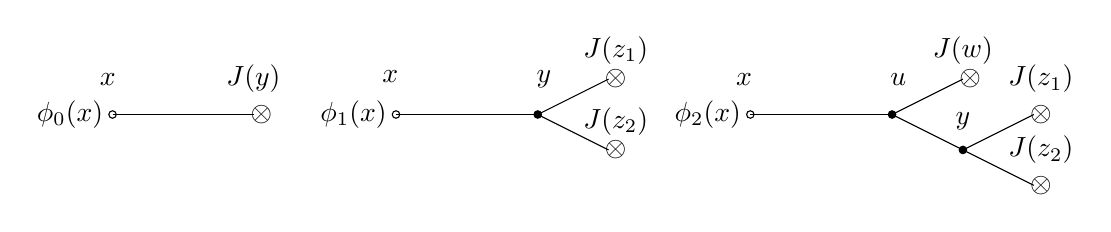
\begin{tikzpicture}[scale=0.9, baseline]
      \draw (0,0) -- (2,0);
	  \draw (0,0) circle (1.5pt);
	  \node at (-0.6,0) [] {$\phi_0(x)$};
	  \node at (0.9,0.5) [] {$\quad x\qquad\qquad J(y)$};
      \node at (2.1,0) [] {$\otimes$};
      
      \draw (4,0) -- (6,0);
	  \draw (4,0) circle (1.5pt);
	  \node at (3.4,0) [] {$\phi_1(x)$};
	  \node at (5,0.5) [] {$x\qquad\qquad\quad y$};
	  \filldraw (6,0) circle (1.5pt);
	        \draw (6,0) -- (7,+0.5);
	        \draw (6,0) -- (7,-0.5);
	  \node at (7.1,+0.9) [] {$J(z_1)$};
	  \node at (7.1,-0.1) [] {$J(z_2)$};
      \node at (7.1,+0.5) [] {$\otimes$};
      \node at (7.1,-0.5) [] {$\otimes$};
      
      \draw (9,0) -- (11,0);
	  \draw (9,0) circle (1.5pt);
	  \node at (8.4,0) [] {$\phi_2(x)$};
	  \node at (10,0.5) [] {$x\qquad\qquad\quad u$};
	  	  \filldraw (11,0) circle (1.5pt);
	        \draw (11,0) -- (12,+0.5);
	        \draw (11,0) -- (12,-0.5);
      \node at (12.1,+0.5) [] {$\otimes$};
      \filldraw (12,-0.5) circle (1.5pt);
      		\draw (12,-0.5) -- (13,+0.0);
      		\draw (12,-0.5) -- (13,-1.0);
	  \node at (12,+0.9) [] {$J(w)$};
	  \node at (12,-0.1) [] {$y$};		
      	  
	  \node at (13.1,+0.5) [] {$J(z_1)$};
	  \node at (13.1,-0.5) [] {$J(z_2)$};		
      \node at (13.1,0) [] {$\otimes$};
      \node at (13.1,-1) [] {$\otimes$};
      
    \end{tikzpicture}
\end{figure}

Now constructing the $\lambda^3$ term $\phi_3(x)$ (three black nodes)
\begin{figure}[!h]
\centering
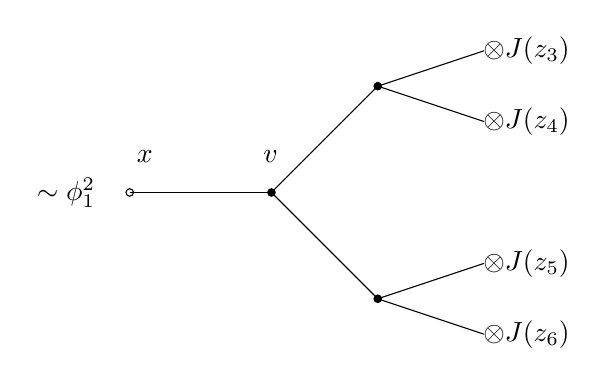
\begin{tikzpicture}[scale=0.9, baseline]
      \draw (0,0) -- (2,0);
	  \draw (0,0) circle (1.5pt);
	  \node at (-0.9,0) [] {$\sim\phi_1^2$};
	  \node at (0.9,0.5) [] {$\quad x\qquad\qquad v$};
	  \filldraw (2,0) circle (1.5pt);
	  \filldraw (3.5,1.5) circle (1.5pt);
	  \filldraw (3.5,-1.5) circle (1.5pt);
      \draw (2,0) -- (3.5,1.5);
      \draw (2,0) -- (3.5,-1.5);
      \draw (3.5,1.5) -- (5,2);
      \draw (3.5,1.5) -- (5,1);
      \draw (3.5,-1.5) -- (5,-2);
      \draw (3.5,-1.5) -- (5,-1);
      \node at (5.6,2) [] {$\otimes J(z_3)$};
      \node at (5.6,1) [] {$\otimes J(z_4)$};
      \node at (5.6,-1) [] {$\otimes J(z_5)$};
      \node at (5.6,-2) [] {$\otimes J(z_6)$};
    \end{tikzpicture}
\end{figure}

\begin{figure}[!h]
\centering
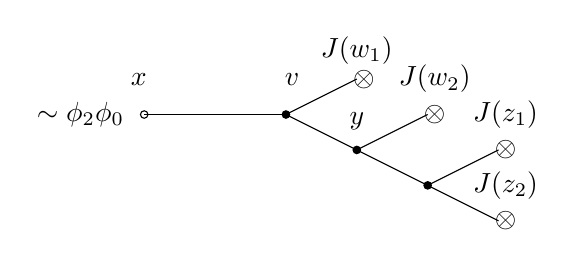
\begin{tikzpicture}[scale=0.9, baseline]
      \draw (9,0) -- (11,0);
	  \draw (9,0) circle (1.5pt);
	  \node at (8.1,0) [] {$\sim\phi_2\phi_0$};
	  \node at (10,0.5) [] {$x\qquad\qquad\quad v$};
	  	  \filldraw (11,0) circle (1.5pt);
	        \draw (11,0) -- (12,+0.5);
	        \draw (11,0) -- (12,-0.5);
      \node at (12.1,+0.5) [] {$\otimes$};
      \filldraw (12,-0.5) circle (1.5pt);
      		\draw (12,-0.5) -- (13,+0.0);
      		\draw (12,-0.5) -- (13,-1.0);
	  \node at (12,+0.9) [] {$J(w_1)$};
	  \node at (12,-0.1) [] {$y$};		
      	  
	  \node at (13.1,+0.5) [] {$J(w_2)$};
      \node at (13.1,0) [] {$\otimes$};
      \filldraw (13,-1) circle (1.5pt);
		\draw (13,-1) -- (14,-0.5);
		\draw (13,-1) -- (14,-1.5);
	  \node at (14.1,-0.0) [] {$J(z_1)$};
	  \node at (14.1,-1.0) [] {$J(z_2)$};		
      \node at (14.1,-0.5) [] {$\otimes$};
      \node at (14.1,-1.5) [] {$\otimes$};
      
    \end{tikzpicture}
\end{figure}

We can also calculate - and obtain the same result
\begin{align}
&\phi_3(x)=(-i)\int dv\,D_F(x-v)\left(2\underbrace{i\int dw_1\,D_F(v-w_1)J(w_1)}_{=\phi_0(v)}\cdot\right.\\
&\cdot\underbrace{\frac{i}{2}\int\!\!\!\int\!\!\!\int\!\!\!\int\!\!\!\int\,du\,dw_2\,dy\,dz_1\,dz_2\,D_F(v-u)D_F(u-w_2)J(w_2)D_F(u-y)D_F(y-z_1)J(z_1)D_F(y-z_2) J(z_2)}_{=\phi_2(v)}+\\
&+\underbrace{\frac{i}{2}\iiint dy_1\,dz_3\,dz_4\,D_F(v-y_1)D_F(y_1-z_3) J(z_3)D_F(y_1-z_4) J(z_4)}_{\phi_1(v)}\cdot\\
&\cdot\left.\underbrace{\frac{i}{2}\iiint dy_2\,dz_5\,dz_6\,D_F(v-y_2)D_F(y_2-z_5) J(z_5)D_F(y_2-z_6) J(z_6)}_{\phi_1(v)}\right)\\
&=i\int dv\,dw_1\,du\,dw_2\,dy\,dz_1\,dz_2\,D_{xv}D_{vw_1}J(w_1)D_{vu}D_{uw_2}J(w_2)D_{uy}D_{yz_1}J(z_1)D_{yz_2} J(z_2)\\
&+\frac{i}{4}\int\,dv\,dy_1\,dz_3\,dz_4\,dy_2\,dz_5\,dz_6\,D_{xv}D_{vy_1}D_{y_1z_3} J(z_3)D_{y_1z_4} J(z_4)D_{vy_2}D_{y_2z_5} J(z_5)D_{y_2z_6} J(z_6)
\end{align}


\item Intuitively we expect only stuff to happen at $\lambda^2$ order because the only relevant (low order) tree level diagrams are.
\begin{figure}[!h]
\centering
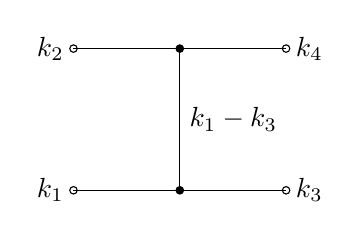
\begin{tikzpicture}[scale=0.9, baseline]
      \draw (0,0) -- (3,0);
      \draw (1.5,0) -- (1.5,2);
      \draw (0,2) -- (3,2);
	  \draw (0,0) circle (1.5pt);
	  \node at (0,0) [left] {$k_1$};
	  \draw (0,2) circle (1.5pt);
	  \node at (0,2) [left] {$k_2$};
	  \draw (3,0) circle (1.5pt);
	  \node at (3,0) [right] {$k_3$};
	  \draw (3,2) circle (1.5pt);
	  \node at (3,2) [right] {$k_4$};
	  \node at (1.5,1) [right] {$k_1-k_3$};
	  \filldraw (1.5,0) circle (1.5pt);
	  \filldraw (1.5,2) circle (1.5pt);
    \end{tikzpicture}
    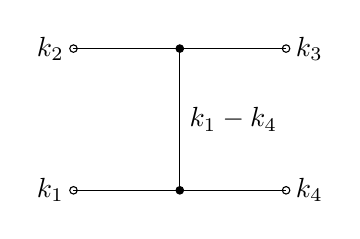
\begin{tikzpicture}[scale=0.9, baseline]
      \draw (0,0) -- (3,0);
      \draw (1.5,0) -- (1.5,2);
      \draw (0,2) -- (3,2);
	  \draw (0,0) circle (1.5pt);
	  \node at (0,0) [left] {$k_1$};
	  \draw (0,2) circle (1.5pt);
	  \node at (0,2) [left] {$k_2$};
	  \draw (3,0) circle (1.5pt);
	  \node at (3,0) [right] {$k_4$};
	  \draw (3,2) circle (1.5pt);
	  \node at (3,2) [right] {$k_3$};
	  \node at (1.5,1) [right] {$k_1-k_4$};
	  \filldraw (1.5,0) circle (1.5pt);
	  \filldraw (1.5,2) circle (1.5pt);
    \end{tikzpicture}
        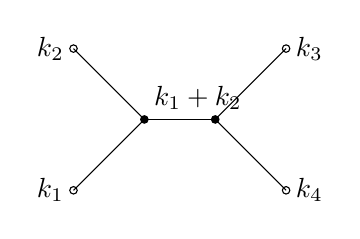
\begin{tikzpicture}[scale=0.9, baseline]
      \draw (0,0) -- (1,1);
      \draw (1,1) -- (2,1);
      \draw (2,1) -- (3,2);
      \draw (0,2) -- (1,1);
      \draw (2,1) -- (3,0);
	  \draw (0,0) circle (1.5pt);
	  \node at (0,0) [left] {$k_1$};
	  \draw (0,2) circle (1.5pt);
	  \node at (0,2) [left] {$k_2$};
	  \draw (3,0) circle (1.5pt);
	  \node at (3,0) [right] {$k_4$};
	  \draw (3,2) circle (1.5pt);
	  \node at (3,2) [right] {$k_3$};
	  \node at (1,1.3) [right] {$k_1+k_2$};
	  \filldraw (1,1) circle (1.5pt);
	  \filldraw (2,1) circle (1.5pt);
    \end{tikzpicture}
\end{figure}
We calculate anyway - so substituting (shortening the notation $D_F(x-y)\equiv D_{xy}$)
\begin{align}
S&_\text{on-shell}[J]
=S[\phi(J)]\\
&=S[\phi_0+\lambda\phi_1+\lambda^2\phi_2+...]\\
&=\int d^4x\left(-\frac{1}{2}(\Box-m^2)(\phi_0+\lambda\phi_1+\lambda^2\phi_2+...)-\frac{\lambda}{3!}(\phi_0+\lambda\phi_1+\lambda^2\phi_2+...)^3+J(\phi_0+\lambda\phi_1+\lambda^2\phi_2+...)\right)\\
&=\int d^4x\left(-\frac{1}{2}(-J+\lambda\frac{1}{2}\phi_0^2+\lambda^2\phi_0\phi_1+...)-\frac{\lambda}{3!}(\phi_0^3+3\phi_1\phi_0^2\lambda+3\phi_0(\phi_1^2+\phi_0\phi_2)\lambda^2+...)+J(\phi_0+\lambda\phi_1+\lambda^2\phi_2+...)\right)\\
&=\int d^4x\, J\left(\phi_0+\frac{1}{4}\right)
+\lambda\int d^4x\left(-\frac{1}{6}\phi_0^2\left[\phi_0+\frac{3}{2}\right]+J\phi_1\right)
+\lambda^2\int d^4x\left(-\frac{1}{2}\phi_0\phi_1(\phi_0+1)+J\phi_2\right)+...
\end{align}
Now we look at the individual contributions (shortening notation) - and doing to first functional integral in baby steps
\begin{align}
S_0&=\int d^4x\, J\left(\phi_0+\frac{1}{4}\right)\\
&=\int dx\, J(x)\left(i\int dy\,D_F(x-y)J(y)+\frac{1}{4}\right)\\
&=\frac{1}{4}\int dx\,J(x)+i\int dx\,dy J(x)D_{xy}J(y)\\
\rightarrow\frac{\delta S_0[J]}{\delta J(x_i)}&=\lim_{\epsilon\rightarrow0}\frac{1}{\epsilon}\left[\frac{1}{4}\int dx\,\left[J(x)+\epsilon\delta(x-x_i)\right]-\frac{1}{4}\int dx\,J(x)\right]\\
&+i\lim_{\epsilon\rightarrow0}\frac{1}{\epsilon}\left[i\int dx\,dy (J(x)+\epsilon\delta(x-x_i))D_{xy}(J(y)+\epsilon\delta(y-x_i))-i\int dx\,dy J(x)D_{xy}J(y)\right]\\
&=\frac{1}{4}\int dx\,\delta(x-x_j)+i\int dx\,dy\left[\delta(x-x_i)D_{xy}J(y)+J(x)D_{xy}\delta(y-x_i)\right]\\
&=\frac{1}{4}+i\int dy\,D_{x_iy}J(y)+i\int dx\,D_{xx_i}J(x)
\end{align}
this terms contains only one $J$ - performing the other three functional derivatives $\delta/\delta J(x_k)$ will result in a zero.

Now we can calculate a bit faster
\begin{align}
S_1&=-\frac{1}{6}\int dx\,\phi_0^3-\frac{1}{4}\int dx\,\phi_0^2+\int dx\,J\phi_1\\
&=-\frac{i^3}{6}\int dx\,dy_1\,dy_2\,dy_3\,D_{xy_3}J(y_3)D_{xy_2}J(y_2)D_{xy_1}J(y_1)
-\frac{i^2}{4}\int dx\,dy_1\,dy_2D_{xy_2}J(y_2)D_{xy_1}J(y_1)\\& 
+\frac{i}{2}\int dx\,dy\,dz_1\,dz_2\,J(x)\,D_{xy}D_{yz_1} J(z_1)D_{yz_2} J(z_2)\\
\rightarrow\frac{\delta S_1[J]}{\delta J(x_i)}
&=-\frac{i^3}{6}\int dx\,dy_1\,dy_2\,D_{xx_i}D_{xy_2}J(y_2)D_{xy_1}J(y_1)
-\frac{i^3}{6}\int dx\,dy_1\,dy_3\,D_{xy_3}J(y_3)D_{xx_i}D_{xy_1}J(y_1)\\
&-\frac{i^3}{6}\int dx\,dy_2\,dy_3\,D_{xy_3}J(y_3)D_{xy_2}J(y_2)D_{xx_1}\\
&-\frac{i^2}{4}\int dx\,dy_1\,D_{xx_i}D_{xy_1}J(y_1)-\frac{i^2}{4}\int dx\,dy_2D_{xy_2}J(y_2)D_{xx_i}\\
&+\frac{i}{2}\int \,dy\,dz_1\,dz_2\,\,D_{x_1y}D_{yz_1} J(z_1)D_{yz_2} J(z_2)
+\frac{i}{2}\int dx\,dy\,dz_2\,J(x)\,D_{xy}D_{yx_1}D_{yz_2} J(z_2)\\
&+\frac{i}{2}\int dx\,dy\,dz_1\,J(x)\,D_{xy}D_{yz_1} J(z_1)D_{yx_i}
\end{align}
this terms contains only two $J$ - performing the other three functional derivatives $\delta/\delta J(x_k)$ will result in a zero.
And
\begin{align}
S_2&=-\frac{1}{2}\int dx\,\phi_0^2\phi_1-\frac{1}{2}\int dx\,\phi_0\phi_1+\int dx\,J(x)\phi_2\\
&=-\frac{i^2}{2}\int dx\,dy_1d\,y_2\,D_{xy_2}J(y_2)D_{xy_1}J(y_1)\frac{i}{2}\iiint d^4y\,d^4z_1\,d^4z_2\,D_{xy}D_{yz_1}J(z_1)D_{yz_2}J(z_2)\\
&-\frac{i^2}{2}\int dx\,dy_1d\,D_{xy_2}J(y_2)\frac{i}{2}\iiint d^4y\,d^4z_1\,d^4z_2\,D_{xy}D_{yz_1}J(z_1)D_{yz_2}J(z_2)\\
&+\int dx\,J(x)\frac{i}{2}\int du\,dw\,dy\,dz_1\,dz_2\,D_{xu}D_{uw}J(w)D_{uy}D_{yz_1}J(z_1)D_{yz_2}J(z_2)\\
&=-\frac{i^3}{4}\int dx\,dy_1d\,y_2\,dy\,dz_1\,dz_2\,D_{xy_2}J(y_2)D_{xy_1}J(y_1) D_{xy}D_{yz_1}J(z_1)D_{yz_2}J(z_2)\\
&+\frac{i}{2}\int dx\,du\,dw\,dy\,dz_1\,dz_2\,\,J(x)D_{xu}D_{uw}J(w)D_{uy}D_{yz_1}J(z_1)D_{yz_2}J(z_2)+\mathcal{O}(J^3)
\end{align}
Now first integral - one derivative
\begin{align}
\frac{\delta}{\delta J(x_1)}&\int dx\,dy_1\,dy_2\,dy\,dz_1\,dz_2\,D_{xy_2}J(y_2)D_{xy_1}J(y_1) D_{xy}D_{yz_1}J(z_1)D_{yz_2}J(z_2)\\
&=\int dx\,dy_1\,dy\,dz_1\,dz_2\,D_{xx_1}D_{xy_1}J(y_1) D_{xy}D_{yz_1}J(z_1)D_{yz_2}J(z_2)\\
&+\int dx\,dy_2\,dy\,dz_1\,dz_2\,D_{xy_2}J(y_2)D_{xx_1} D_{xy}D_{yz_1}J(z_1)D_{yz_2}J(z_2)\\
&+\int dx\,dy_1\,dy_2\,dy\,dz_2\,D_{xy_2}J(y_2)D_{xy_1}J(y_1) D_{xy}D_{yx_1}D_{yz_2}J(z_2)\\
&+\int dx\,dy_1\,dy_2\,dy\,dz_1\,D_{xy_2}J(y_2)D_{xy_1}J(y_1) D_{xy}D_{yz_1}J(z_1)D_{yz_1}
\end{align}
two derivatives
\begin{align}
\frac{\delta}{\delta J(x_2)}\frac{\delta}{\delta J(x_1)}\int dx\,dy_1\,dy_2\,dy\,dz_1\,dz_2\,D_{xy_2}J(y_2)D_{xy_1}J(y_1) D_{xy}D_{yz_1}J(z_1)D_{yz_2}J(z_2)\\
=+\int dx\,dy\,dz_1\,dz_2\,D_{xx_1}D_{xx_2} D_{xy}D_{yz_1}J(z_1)D_{yz_2}J(z_2)\\
+\int dx\,dy_1\,dy\,dz_2\,D_{xx_1}D_{xy_1}J(y_1) D_{xy}D_{yx_2}D_{yz_2}J(z_2)\\
+\int dx\,dy_1\,dy\,dz_1\,D_{xx_1}D_{xy_1}J(y_1) D_{xy}D_{yz_1}J(z_1)D_{yx_2}\\
%
+\int dx\,dy_2\,dy\,dz_2\,D_{xy_2}J(y_2)D_{xx_1} D_{xy}D_{yx_2}D_{yz_2}J(z_2)\\
+\int dx\,dy\,dz_1\,dz_2\,D_{xx_2}D_{xx_1} D_{xy}D_{yz_1}J(z_1)D_{yz_2}J(z_2)\\
+\int dx\,dy_2\,dy\,dz_1\,D_{xy_2}J(y_2)D_{xx_1} D_{xy}D_{yz_1}J(z_1)D_{yx_2}\\
%
+\int dx\,dy_1\,dy\,dz_2\,D_{xx_2})D_{xy_1}J(y_1) D_{xy}D_{yx_1}D_{yz_2}J(z_2)\\
+\int dx\,dy_2\,dy\,dz_2\,D_{xy_2}J(y_2)D_{xx_2} D_{xy}D_{yx_1}D_{yz_2}J(z_2)\\
+\int dx\,dy_1\,dy_2\,dy\,D_{xy_2}J(y_2)D_{xy_1}J(y_1) D_{xy}D_{yx_1}D_{yx_2}\\
%
+\int dx\,dy_1\,dy\,dz_1\,D_{xx_2}D_{xy_1}J(y_1) D_{xy}D_{yz_1}J(z_1)D_{yz_1}\\
+\int dx\,dy_2\,dy\,dz_1\,D_{xy_2}J(y_2)D_{xx_2} D_{xy}D_{yz_1}J(z_1)D_{yz_1}\\
+\int dx\,dy_1\,dy_2\,dy\,D_{xy_2}J(y_2)D_{xy_1}J(y_1) D_{xy}D_{yx_2}D_{yz_1}
\end{align}
three derivatives
\begin{align}
\frac{\delta}{\delta J(x_3)}\frac{\delta}{\delta J(x_2)}\frac{\delta}{\delta J(x_1)}\int dx\,dy_1\,dy_2\,dy\,dz_1\,dz_2\,D_{xy_2}J(y_2)D_{xy_1}J(y_1) D_{xy}D_{yz_1}J(z_1)D_{yz_2}J(z_2)\\
=+\int dx\,dy\,dz_2\,D_{xx_1}D_{xx_2} D_{xy}D_{yx_3}D_{yz_2}J(z_2)
+\int dx\,dy\,dz_1\,D_{xx_1}D_{xx_2} D_{xy}D_{yz_1}J(z_1)D_{yx_3}\\
%
+\int dx\,dy\,dz_2\,D_{xx_1}D_{xx_3} D_{xy}D_{yx_2}D_{yz_2}J(z_2)
+\int dx\,dy_1\,dy\,D_{xx_1}D_{xy_1}J(y_1) D_{xy}D_{yx_2}D_{yx_3}\\
%
+\int dx\,dy\,dz_1\,D_{xx_1}D_{xx_3} D_{xy}D_{yz_1}J(z_1)D_{yx_2}
+\int dx\,dy_1\,dy\,D_{xx_1}D_{xy_1}J(y_1) D_{xy}D_{yx_3}D_{yx_2}\\
%
+\int dx\,dy\,dz_2\,D_{xx_3}D_{xx_1} D_{xy}D_{yx_2}D_{yz_2}J(z_2)
+\int dx\,dy_2\,dy\,D_{xy_2}J(y_2)D_{xx_1} D_{xy}D_{yx_2}D_{yx_3}\\
%
+\int dx\,dy\,dz_2\,D_{xx_2}D_{xx_1} D_{xy}D_{yx_3}D_{yz_2}J(z_2)
+\int dx\,dy\,dz_1\,D_{xx_2}D_{xx_1} D_{xy}D_{yz_1}J(z_1)D_{yx_3}\\
%
+\int dx\,dy\,dz_1\,D_{xx_3}D_{xx_1} D_{xy}D_{yz_1}J(z_1)D_{yx_2}
+\int dx\,dy_2\,dy\,D_{xy_2}J(y_2)D_{xx_1} D_{xy}D_{yx_3}D_{yx_2}\\
%
+\int dx\,dy\,dz_2\,D_{xx_2})D_{xx_3} D_{xy}D_{yx_1}D_{yz_2}J(z_2)
+\int dx\,dy_1\,dy\,D_{xx_2})D_{xy_1}J(y_1) D_{xy}D_{yx_1}D_{yx_3}\\
%
+\int dx\,dy\,dz_2\,D_{xx_3}D_{xx_2} D_{xy}D_{yx_1}D_{yz_2}J(z_2)
+\int dx\,dy_2\,dy\,D_{xy_2}J(y_2)D_{xx_2} D_{xy}D_{yx_1}D_{yx_3}\\
%
+\int dx\,dy_1\,dy\,D_{xx_3}D_{xy_1}J(y_1) D_{xy}D_{yx_1}D_{yx_2}
+\int dx\,dy_2\,dy\,D_{xy_2}J(y_2)D_{xx_3}D_{xy}D_{yx_1}D_{yx_2}\\
%
+\int dx\,dy\,dz_1\,D_{xx_2}D_{xx_3} D_{xy}D_{yz_1}J(z_1)D_{yz_1}
+\int dx\,dy_1\,dy\,D_{xx_2}D_{xy_1}J(y_1) D_{xy}D_{yx_3}D_{yz_1}\\
%
+\int dx\,dy\,dz_1\,D_{xx_3}D_{xx_2} D_{xy}D_{yz_1}J(z_1)D_{yz_1}
+\int dx\,dy_2\,dy\,D_{xy_2}J(y_2)D_{xx_2} D_{xy}D_{yx_3}D_{yz_1}\\
%
+\int dx\,dy_2\,dy\,D_{xx_3}D_{xy_1}J(y_1) D_{xy}D_{yx_2}D_{yz_1}
+\int dx\,dy_1\,dy\,D_{xy_2}J(y_2)D_{xx_3} D_{xy}D_{yx_2}D_{yz_1}
\end{align}
four derivatives
\begin{align}
\frac{\delta}{\delta J(x_4)}\frac{\delta}{\delta J(x_3)}\frac{\delta}{\delta J(x_2)}\frac{\delta}{\delta J(x_1)}\int dx\,dy_1\,dy_2\,dy\,dz_1\,dz_2\,D_{xy_2}J(y_2)D_{xy_1}J(y_1) D_{xy}D_{yz_1}J(z_1)D_{yz_2}J(z_2)\\
=+\int dx\,dy\,D_{xx_1}D_{xx_2} D_{xy}D_{yx_3}D_{yx_4}
+\int dx\,dy\,D_{xx_1}D_{xx_2} D_{xy}D_{yx_4}D_{yx_3}\\
%
+\int dx\,dy\,D_{xx_1}D_{xx_3} D_{xy}D_{yx_2}D_{yx_4}
+\int dx\,dy\,D_{xx_1}D_{xx_4} D_{xy}D_{yx_2}D_{yx_3}\\
%
+\int dx\,dy\,D_{xx_1}D_{xx_3} D_{xy}D_{yx_4}D_{yx_2}
+\int dx\,dy\,D_{xx_1}D_{xx_4} D_{xy}D_{yx_3}D_{yx_2}\\
%
+\int dx\,dy\,D_{xx_3}D_{xx_1} D_{xy}D_{yx_2}D_{yx_4}
+\int dx\,dy\,D_{xx_4}D_{xx_1} D_{xy}D_{yx_2}D_{yx_3}\\
%
+\int dx\,dy\,D_{xx_2}D_{xx_1} D_{xy}D_{yx_3}D_{yx_4}
+\int dx\,dy\,D_{xx_2}D_{xx_1} D_{xy}D_{yx_4}D_{yx_3}\\
%
+\int dx\,dy\,D_{xx_3}D_{xx_1} D_{xy}D_{yx_4}D_{yx_2}
+\int dx\,dy\,D_{xx_4}D_{xx_1} D_{xy}D_{yx_3}D_{yx_2}\\
%
+\int dx\,dy\,D_{xx_2}D_{xx_3} D_{xy}D_{yx_1}D_{yx_4}
+\int dx\,dy\,D_{xx_2}D_{xx_4} D_{xy}D_{yx_1}D_{yx_3}\\
%
+\int dx\,dy\,D_{xx_3}D_{xx_2} D_{xy}D_{yx_1}D_{yx_4}
+\int dx\,dy\,D_{xx_4}D_{xx_2} D_{xy}D_{yx_1}D_{yx_3}\\
%
+\int dx\,dy\,D_{xx_3}D_{xx_4}D_{xy}D_{yx_1}D_{yx_2}
+\int dx\,dy\,D_{xx_4}D_{xx_3}D_{xy}D_{yx_1}D_{yx_2}\\
%
+\int dx\,dy\,D_{xx_2}D_{xx_3} D_{xy}D_{yx_4}D_{yz_1}
+\int dx\,dy\,D_{xx_2}D_{xx_4}D_{xy}D_{yx_3}D_{yz_1}\\
%
+\int dx\,dy\,D_{xx_3}D_{xx_2} D_{xy}D_{yx_4}D_{yz_1}
+\int dx\,dy\,D_{xx_4}D_{xx_2} D_{xy}D_{yx_3}D_{yz_1}\\
%
+\int dx\,dy\,D_{xx_3}D_{xx_4} D_{xy}D_{yx_2}D_{yz_1}
+\int dx\,dy\,D_{xx_4}D_{xx_3} D_{xy}D_{yx_2}D_{yz_1}
\end{align}

\begin{align*}
\frac{\delta}{\delta J(x_4)}\frac{\delta}{\delta J(x_3)}\frac{\delta}{\delta J(x_2)}\frac{\delta}{\delta J(x_1)}\int dx\,dy_1\,dy_2\,dy\,dz_1\,dz_2\,D_{xy_2}J(y_2)D_{xy_1}J(y_1) D_{xy}D_{yz_1}J(z_1)D_{yz_2}J(z_2)\\
=4\int dx\,dy\,D_{xx_1}D_{xx_2} D_{xy}D_{yx_3}D_{yx_4}
+4\int dx\,dy\,D_{xx_1}D_{xx_3} D_{xy}D_{yx_2}D_{yx_4}
+4\int dx\,dy\,D_{xx_1}D_{xx_4} D_{xy}D_{yx_2}D_{yx_3}\\
+4\int dx\,dy\,D_{xx_2}D_{xx_3} D_{xy}D_{yx_1}D_{yx_4}
+4\int dx\,dy\,D_{xx_2}D_{xx_4} D_{xy}D_{yx_1}D_{yx_3}
+4\int dx\,dy\,D_{xx_3}D_{xx_4} D_{xy}D_{yx_3}D_{yx_4}
\end{align*}
\end{enumerate}
Second integral - analog calculation
\begin{align}
\frac{\delta}{\delta J(x_4)}\frac{\delta}{\delta J(x_3)}\frac{\delta}{\delta J(x_2)}\frac{\delta}{\delta J(x_1)}\int dx\,du\,dw\,dy\,dz_1\,dz_2\,\,J(x)D_{xu}D_{uw}J(w)D_{uy}D_{yz_1}J(z_1)D_{yz_2}J(z_2)\\
=2\int du\,dy\,\,D_{x_1u}D_{ux_2}D_{uy}D_{yx_3}D_{yx_4}
+2\int du\,dy\,\,D_{x_2u}D_{ux_2}D_{uy}D_{yx_3}D_{yx_4}
+2\int du\,dy\,\,D_{x_1u}D_{ux_3}D_{uy}D_{yx_2}D_{yx_4}\\
+2\int du\,dy\,\,D_{x_3u}D_{ux_1}D_{uy}D_{yx_2}D_{yx_4}
+2\int du\,dy\,\,D_{x_1u}D_{ux_4}D_{uy}D_{yx_2}D_{yx_3}
+2\int du\,dy\,\,D_{x_4u}D_{ux_1}D_{uy}D_{yx_2}D_{yx_3}\\
+2\int du\,dy\,\,D_{x_2u}D_{ux_3}D_{uy}D_{yx_1}D_{yx_4}
+2\int du\,dy\,\,D_{x_3u}D_{ux_2}D_{uy}D_{yx_1}D_{yx_4}
+2\int du\,dy\,\,D_{x_2u}D_{ux_4}D_{uy}D_{yx_1}D_{yx_3}\\
+2\int du\,dy\,\,D_{x_4u}D_{ux_2}D_{uy}D_{yx_1}D_{yx_3}
+2\int du\,dy\,\,D_{x_3u}D_{ux_4}D_{uy}D_{yx_1}D_{yx_2}
+2\int du\,dy\,\,D_{x_4u}D_{ux_3}D_{uy}D_{yx_1}D_{yx_2}
\end{align}
This last two expression is all that survives the funtional derivatives and setting $J\rightarrow0$. 

Now we can calculate one example term of the first integral using the Klein-Gordon Greens function property of the Feynman propagator $(\Box_{x}-m^2)D_F(x-y)=i\delta^{(4)}(x-y)$
\begin{align}
\int d^4x_1\,e^{i(k_1x_1)}(\Box_{x_1}-m^2)\int dx\,dy\,D_{xx_1}D_{xx_2} D_{xy}D_{yx_3}D_{yx_4}
&=\int dx\,dy\,e^{i(k_1x_1)}\,(-i)\delta^{(4)}(x-x_1)D_{xx_2} D_{xy}D_{yx_3}D_{yx_4}\\
&=-i\int dx\,dy\,e^{i(k_1x)}\,D_{xx_2} D_{xy}D_{yx_3}D_{yx_4}
\end{align}
so we can generalize to the $x_1, x_2, x_3, x_4$ integration - and do the Fourier trafo of the Feynman propagator (via substitution $u=x-y, v=y$, meaning $x=u+v, y=v, dxdy=dudv $)
\begin{align}
\int \prod_{i=1}^4d^4x_i\,e^{i(k_ix_i)}(\Box_{x_i}-m^2)\int dx\,dy\,D_{xx_1}D_{xx_2} D_{xy}D_{yx_3}D_{yx_4}
&=(-i)^4\int \,dx\,dy\,e^{i(k_1x+k_2x+k_3y+k_4y)}D_{xy}\\
&=\int \,dx\,dy\,e^{i(k_1+k_2)x+i(k_3+k_4)y}D_F(x-y)\\
&=\int \,du\,dv\,e^{i(k_1+k_2)(u+v)+i(k_3+k_4)v}D_F(u)\\
&=\int dv\,e^{i(k_1+k_2+k_3+k_4)v}\cdot\int \,du\,e^{i(k_1+k_2)u}D_F(u)\\
&=(2\pi)^4\delta^{(4)}(k_1+k_2+k_3+k_4)\frac{i}{(k_1+k_2)^2-m^2+i\epsilon}
\end{align}
we see that all the 6 different terms end up in the similar expression.

Now we can do one term of the second integral
\begin{align}
\int \prod_{i=1}^4d^4x_i\,e^{i(k_ix_i)}(\Box_{x_i}-m^2)\int du\,dy\,\,D_{x_1u}D_{ux_2}D_{uy}D_{yx_3}D_{yx_4}
&=(-i)^4\int du\,dy\,e^{i(k_1u+k_2u+k_3y+k_4y)}D_F(u-y)\\
&=(-i)^4\int du\,dy\,e^{i(k_1+k_2)u}e^{i(k_3+k_4)y}D_F(u-y)\\
&=(2\pi)^4\delta^{(4)}(k_1+k_2+k_3+k_4)\frac{i}{(k_1+k_2)^2-m^2+i\epsilon}
\end{align}
So in total we should get three types of terms for the pairs (s, t, u-channels) $k_1,k_2$ and $k_1,k_3$ and $k_1,k_4$ (I would need some more time to collect all prefactors)
\begin{align}
\int \prod_{i=1}^4d^4x_i\,e^{i(k_ix_i)}(\Box_{x_i}-m^2)\left.\frac{\delta}{\delta J(x_i)}S[(J)]\right|_{J=0}
=\lambda^2\int \prod_{i=1}^4d^4x_i\,e^{i(k_ix_i)}(\Box_{x_i}-m^2)\left.\frac{\delta}{\delta J(x_i)}S_2[(J)]\right|_{J=0}\\
\sim\lambda^2(2\pi)^{4}\delta^{(4)}(k_1+k_2+k_3+k_4)\left(\frac{1}{(k_1+k_2)^2-m^2}+\frac{1}{(k_1+k_3)^2-m^2}+\frac{1}{(k_1+k_4)^2-m^2}\right)
\end{align}
\newpage

\section{Quantum Field Theory II – Exercise sheet 2 (2025-06-11)}
\subsection{Exercise 1 - Dimensional Regularization in QED}

{\color{blue} We consider the 1-loop vacuum polarization discussed in the lecture, for which we found
\begin{align}
\Pi_2^{\mu\nu}
&=-4ie^2\int\frac{d^4k}{(2\pi)^4}\frac{2k^\mu k^\nu-\eta^{\mu\nu}(k^2-p\cdot k+m^2)}{[(k-p)^2+m^2][k^2+m^2]} \tag{1}
\end{align}
Our goal is to compute this 1-loop integral in dimensional regularization.
\begin{enumerate}
\item Use the Feynman parameter trick to write the integral with a denominator that is a complete square.

\item Prove
\begin{align}
\int\frac{d^Dk}{(2\pi)^D}\frac{k^{2a}}{(k^2-\Delta)^b}
&=i(-1)^{a-b}\frac{1}{(4\pi)^{D/2}}\frac{1}{\Delta^{b-a-\frac{D}{2}}}\frac{\Gamma\left(a+\frac{D}{2}\right)\Gamma\left(b-a-\frac{D}{2}\right)}{\Gamma\left(b\right)\Gamma\left(\frac{D}{2}\right)} \tag{2}
\end{align}
where $\Gamma$ is the Euler gamma function, and write out the special cases $a= 0,b=2$ and $a=1,b=2$.

\item Compute (1) in dimensional regularization setting $D = 4-\epsilon$. Give the result in the limit $p^2\gg m^2$.
\end{enumerate}
}
\begin{enumerate}[1.]
\item
\begin{enumerate}[1.)]
\item With the observation
\begin{align}
\frac{1}{AB}&=\int_0^1\frac{1}{[At+B(1-t)]^2}dt
\end{align}
we can write
\begin{align}
\rightarrow \frac{2k^\mu k^\nu-\eta^{\mu\nu}(k^2-p\cdot k+m^2)}{[(k-p)^2+m^2][k^2+m^2]} 
&=\int_0^1 dt \frac{2k^\mu k^\nu-\eta^{\mu\nu}(k^2-p\cdot k+m^2)}{([(k-p)^2+m^2]t+[k^2+m^2](1-t))^2}\\
&=\int_0^1 dt \frac{2k^\mu k^\nu-\eta^{\mu\nu}(k^2-p\cdot k+m^2)}{([k^2-2kp+p^2+m^2]t+[k^2+m^2](1-t))^2}\\
&=\int_0^1 dt \frac{2k^\mu k^\nu-\eta^{\mu\nu}(k^2-p\cdot k+m^2)}{(k^2-2kpt+p^2t+m^2)^2}\\
&=\int_0^1 dt \frac{2k^\mu k^\nu-\eta^{\mu\nu}(k^2-p\cdot k+m^2)}{([k-pt]^2-p^2t^2+p^2t+m^2)^2}\\
&=\int_0^1 dt \frac{2k^\mu k^\nu-\eta^{\mu\nu}(k^2-p\cdot k+m^2)}{([k-pt]^2+p^2t(1-t)+m^2)^2}
\end{align}
then with $q^\mu=k^\mu-p^\mu t$ and $\Delta=-(p^2t(1-t)+m^2)=p^2t(t-1)-m^2$
\begin{align}
\rightarrow &\frac{2k^\mu k^\nu-\eta^{\mu\nu}(k^2-p\cdot k+m^2)}{[(k-p)^2+m^2][k^2+m^2]} 
=\int_0^1 dt \frac{2(q^\mu+p^\mu t)(q^\nu+p^\nu t)-\eta^{\mu\nu}[(q+pt)^2-p(q+pt)+m^2]}{(q^2-\Delta)^2}\\
&=\int_0^1 dt \frac{2(q^\mu q^\nu+(p^\mu q^\nu+p^\nu q^\mu) t+p^\mu p^\nu t^2)-\eta^{\mu\nu}[q^2+2q\cdot p t+p^2 t^2-p\cdot q-p^2t+m^2]}{(q^2-\Delta)^2}\\
&=\int_0^1 dt \frac{2(q^\mu q^\nu+(p^\mu q^\nu+p^\nu q^\mu) t+p^\mu p^\nu t^2)-\eta^{\mu\nu}[q^2+q\cdot p(2t-1)+p^2(t-1)t+m^2]}{(q^2-\Delta)^2}
\end{align}
we have with $d^4q=d^4k$ (the momentum shift does not change the integral measure)
\begin{align}
\Pi_2^{\mu\nu}
&=-4ie^2\int\frac{d^4k}{(2\pi)^4}\frac{2k^\mu k^\nu-\eta^{\mu\nu}(k^2-p\cdot k+m^2)}{[(k-p)^2+m^2][k^2+m^2]}\\
&=-4ie^2\int_0^1 dt\int\frac{d^4q}{(2\pi)^4} \frac{2(q^\mu q^\nu+(p^\mu q^\nu+p^\nu q^\mu) t+p^\mu p^\nu t^2)-\eta^{\mu\nu}[q^2+q\cdot p(2t-1)+p^2(t-1)t+m^2]}{(q^2-\Delta)^2}
\end{align}
Since the denominator is rotationally symmetric in $q$ so the linear terms are vanishing (see substitution $q\rightarrow-q: d^4q\,q f(q^2)= 0$)
\begin{align}
\Pi_2^{\mu\nu}
&=-4ie^2\int_0^1 dt\int\frac{d^4q}{(2\pi)^4} \frac{2(q^\mu q^\nu+\cancel{(p^\mu q^\nu+p^\nu q^\mu)}t+p^\mu p^\nu t^2)-\eta^{\mu\nu}[q^2+\cancel{q\cdot p}(2t-1)+p^2(t-1)t+m^2]}{(q^2-\Delta)^2}\\
&=-4ie^2\int_0^1 dt\int\frac{d^4q}{(2\pi)^4} \frac{2(q^\mu q^\nu+p^\mu p^\nu t^2)-\eta^{\mu\nu}[q^2+p^2(t-1)t+m^2]}{(q^2-\Delta)^2}
\end{align}
now we can split-off the $q^2$-part of the integrand (for the dimensional regularization it is important to leave the $q^\mu q^\nu$-part untouched for now)
\begin{align}
\Pi_2^{\mu\nu}
&=-4ie^2\int_0^1 dt\int\frac{d^4q}{(2\pi)^4} \frac{2p^\mu p^\nu t^2+2q^\mu q^\nu-\eta^{\mu\nu}[q^2+p^2(t-1)t+m^2]}{(q^2-\Delta)^2}\\
&=-4ie^2\int_0^1 dt\int\frac{d^4q}{(2\pi)^4} \frac{2p^\mu p^\nu t^2-\eta^{\mu\nu}[p^2(t-1)t+m^2]}{(q^2-\Delta)^2}-4ie^2\int_0^1 dt\int\frac{d^4q}{(2\pi)^4}\frac{2q^\mu q^\nu-\eta^{\mu\nu}q^2}{(q^2-\Delta)^2}
\end{align}
Now we can split-off the elementary $t$-integration (marking the \textcolor{red}{$p^\mu p^\nu$} part in \textcolor{red}{red})
\begin{align}
\Pi_2^{\mu\nu}
&=\textcolor{red}{-4ie^2(2p^\mu p^\nu)\int_0^1 dt\, t^2\int\frac{d^4q}{(2\pi)^4} \frac{1}{(q^2-\Delta)^2}}
-4ie^2\eta^{\mu\nu}\int_0^1 dt\,(p^2(1-t)t-m^2)\int\frac{d^4q}{(2\pi)^4} \frac{1}{(q^2-\Delta)^2}\\
&\quad-4ie^2\int_0^1 dt\int\frac{d^4q}{(2\pi)^4}\frac{2q^\mu q^\nu-\eta^{\mu\nu}q^2}{(q^2-\Delta)^2}
\end{align}

\item The surface and volume of $D$-dimensional unit sphere are given by $S_{D-1}=D\cdot V_D=\frac{2\pi^{D/2}}{\Gamma(\frac{D}{2})}$ (from the old the standard trick converting of $D$-dimensional Gauss integral spherical coordinates and recognizing the Gamma function in the radial integration).
\begin{align}
\int\frac{d^Dk}{(2\pi)^D}\frac{k^{2a}}{(k^2-\Delta)^b}
&=\frac{1}{(2\pi)^D} \int d^{D-1}\Omega \int_0^\infty dk\,k^{D-1}\frac{k^{2a}}{(k^2-\Delta)^b}\\
&=\frac{1}{(2\pi)^D} \frac{1}{(-\Delta)^b} \frac{2\pi^{D/2}}{\Gamma(\frac{D}{2})} \int_0^\infty dk\,\frac{k^{2a+D-1}}{(1-k^2/\Delta)^b}\\
&=\frac{1}{2^{D-1}\pi^{D/2}} \frac{1}{(-1)^b\Delta^b} \frac{1}{\Gamma(\frac{D}{2})} \int_0^\infty dk\,\frac{k^{2a+D-1}}{(1-k^2/\Delta)^b}\\
&\overset{q^2=k^2/\Delta }{=}\frac{1}{2^{D-1}\pi^{D/2}} \frac{1}{(-1)^b\Delta^b} \frac{1}{\Gamma(\frac{D}{2})} \Delta^{(2a+D-1)/2+1/2}\int_0^\infty dq\,\frac{q^{2a+D-1}}{(1-q^2)^b}\\
&=\frac{1}{2^{D-1}\pi^{D/2}} \frac{1}{(-1)^b\Delta^{b-a-D/2}} \frac{1}{\Gamma(\frac{D}{2})} \int_0^\infty dq\,\frac{q^{2a+D-1}}{(1-q^2)^b}\\
&\overset{q=iy}{=}\frac{1}{2^{D-1}\pi^{D/2}} \frac{1}{\Delta^{b-a-D/2}} \frac{1}{\Gamma(\frac{D}{2})}(-1)^{a}(-1)^{-b}i \int_0^\infty dy\,\frac{y^{2a+D-1}}{(1+y^2)^b}\\
&=\frac{1}{2^{D-1}\pi^{D/2}} \frac{1}{\Delta^{b-a-D/2}} \frac{1}{\Gamma(\frac{D}{2})}(-1)^{a}(-1)^{-b}i \frac{\Gamma(a+\frac{D}{2})\Gamma(b-a-\frac{D}{2})}{2\Gamma(b)}\\
&=\frac{1}{(4\pi)^{D/2}} \frac{1}{\Delta^{b-a-D/2}}(-1)^{a-b}i \frac{\Gamma(a+\frac{D}{2})\Gamma(b-a-\frac{D}{2})}{\Gamma(b)\Gamma(\frac{D}{2})}
\end{align}



Using $\Gamma(2)=1$ and $\Gamma\left(1+\frac{D}{2}\right)=\frac{D}{2}\Gamma\left(\frac{D}{2}\right)$
\begin{itemize}
\item Special case $a=0, b=2$
\begin{align}
\int\frac{d^Dk}{(2\pi)^D}\frac{1}{(k^2-\Delta)^2}
&=\frac{i}{(4\pi)^{D/2}}\frac{1}{\Delta^{2-\frac{D}{2}}}\Gamma\left(2-\frac{D}{2}\right)
\end{align}

\item Special case $a=1, b=2$
\begin{align}
\int\frac{d^Dk}{(2\pi)^D}\frac{k^{2}}{(k^2-\Delta)^2}
&=-\frac{i}{(4\pi)^{D/2}}\frac{1}{\Delta^{1-\frac{D}{2}}}\frac{\Gamma\left(1+\frac{D}{2}\right)\Gamma\left(1-\frac{D}{2}\right)}{\Gamma\left(\frac{D}{2}\right)}\\
&=-\frac{i}{(4\pi)^{D/2}}\frac{1}{\Delta^{1-\frac{D}{2}}}\frac{D}{2}\,\Gamma\left(1-\frac{D}{2}\right)
\end{align}

\end{itemize}

\item With
\begin{align}
\int\frac{d^{4-\epsilon}k}{(2\pi)^{4-\epsilon}}\frac{1}{(k^2-\Delta)^2}
&=\frac{i}{(4\pi)^{{2-\epsilon}/2}}\frac{1}{\Delta^{2-\frac{{4-\epsilon}}{2}}}\Gamma\left(2-\frac{{4-\epsilon}}{2}\right)\\
&=\frac{i}{(4\pi)^{{2-\epsilon}/2}}\frac{1}{\Delta^{\frac{\epsilon}{2}}}\Gamma\left(\frac{\epsilon}{2}\right)\\
\int\frac{d^{4-\epsilon}k}{(2\pi)^{4-\epsilon}}\frac{k^{2}}{(k^2-\Delta^2)^2}
&=-\frac{i}{(4\pi)^{{2-\epsilon}/2}}\frac{1}{\Delta^{1-\frac{{4-\epsilon}}{2}}}\left(\frac{{4-\epsilon}}{2}\right)\,\Gamma\left(1-\frac{{4-\epsilon}}{2}\right)\\
&=-\frac{i}{(4\pi)^{{2-\epsilon}/2}}\frac{1}{\Delta^{\frac{\epsilon}{2}-1}}\left(2-\frac{\epsilon}{2}\right)\,\Gamma\left(\frac{\epsilon}{2}-1\right)
\end{align}
we can simplify with $q^\mu q^\nu=\frac{q^2}{D}\eta^{\mu\nu}$ and write the integrals in dimensional regularization and introducing a mass-dimension parameter $\mu$ and $D=4-\epsilon$
\begin{align}
\Pi_2^{\mu\nu}
&=\textcolor{red}{-4ie^2(2p^\mu p^\nu)\int_0^1 dt\, t^2\int\frac{d^4q}{(2\pi)^4} \frac{1}{(q^2-\Delta)^2}}
-4ie^2\eta^{\mu\nu}\int_0^1 dt\,(p^2(1-t)t-m^2)\int\frac{d^4q}{(2\pi)^4} \frac{1}{(q^2-\Delta)^2}\\
&\quad-4i\left(\frac{2}{D}-1\right)e^2\eta^{\mu\nu}\int_0^1 dt\int\frac{d^4q}{(2\pi)^4}\frac{q^2}{(q^2-\Delta)^2}\\
%
&=\textcolor{red}{-4ie^2\mu^\epsilon(2p^\mu p^\nu)\frac{i}{(4\pi)^{{2-\epsilon}/2}}\Gamma\left(\frac{\epsilon}{2}\right)\int_0^1 dt\,\frac{t^2}{\Delta^{\frac{\epsilon}{2}}}}
-4ie^2\mu^\epsilon\eta^{\mu\nu}\frac{i}{(4\pi)^{{2-\epsilon}/2}}\Gamma\left(\frac{\epsilon}{2}\right)\int_0^1 dt\,\frac{p^2(1-t)t-m^2}{\Delta^{\frac{\epsilon}{2}}}\\
&\quad-4ie^2\mu^\epsilon\left(\frac{2}{4-\epsilon}-1\right)\eta^{\mu\nu}\frac{-i}{(4\pi)^{{2-\epsilon}/2}}\left(2-\frac{\epsilon}{2}\right)\,\Gamma\left(\frac{\epsilon}{2}-1\right)\int_0^1 dt \frac{1}{\Delta^{\frac{\epsilon}{2}-1}}\\
&=\textcolor{red}{(p^\mu p^\nu)\frac{8e^2\mu^\epsilon}{(4\pi)^{{2-\epsilon}/2}}\Gamma\left(\frac{\epsilon}{2}\right)\int_0^1 dt\,\frac{t^2}{\Delta^{\frac{\epsilon}{2}}}}
+\eta^{\mu\nu}\frac{4e^2\mu^\epsilon}{(4\pi)^{{2-\epsilon}/2}}\Gamma\left(\frac{\epsilon}{2}\right)\int_0^1 dt\,\frac{p^2(1-t)t-m^2}{\Delta^{\frac{\epsilon}{2}}}\\
&\quad-\eta^{\mu\nu}\frac{4e^2\mu^\epsilon}{(4\pi)^{{2-\epsilon}/2}}\left(\frac{\epsilon-2}{2}\right)\,\Gamma\left(\frac{\epsilon}{2}-1\right)\int_0^1 dt \frac{1}{\Delta^{\frac{\epsilon}{2}-1}}
\end{align}
For the limit we use the following series expansions
\begin{align}
\mu^\epsilon&=1+ \log(\mu)\epsilon +\frac{1}{2}\log^2(\mu )\epsilon^2+...\\
\frac{1}{(4\pi)^{2-\epsilon/2}}
&=\frac{1}{(4\pi)^2}\left(1+\frac{1}{2}\log (4\pi)\epsilon+\frac{1}{8}\log^2(4\pi) \epsilon^2+...\right)\\
\Gamma\left(\frac{\epsilon}{2}\right)
&=\frac{2}{\epsilon}-\gamma_{EM}+\frac{1}{24}(6\gamma_{EM}^2+\pi^2)\epsilon+\frac{1}{24}[-\gamma_{EM}^3-\gamma_{EM}\frac{\pi^2}{2}+\psi^{(2)}(1)]\epsilon^2+...\\
\Gamma\left(\frac{\epsilon}{2}-1\right)
&=-\frac{2}{\epsilon }+(\gamma_{EM} -1)+\frac{1}{24} \left(-12+12 \gamma_{EM} -6 \gamma_{EM}^2-\pi^2\right) \epsilon +...\\
\frac{1}{\Delta^{\epsilon/2}}&=1-\frac{1}{2}\log(\Delta)\epsilon+\frac{1}{8}\log^2(\Delta)\epsilon^2+...
\end{align}
which gives combined
\begin{align}
\frac{\mu^\epsilon}{(4\pi)^{-\epsilon/2}}\Gamma\left(\frac{\epsilon}{2}\right)
&=\frac{2}{\epsilon }+[2\log(\mu )-\gamma_{EM} +\log (4\pi)]+O\left(\epsilon \right)\\
&=\frac{2}{\epsilon }+[\log(\mu^2)+\log(e^{-\gamma_{EM}}) +\log (4\pi)]+O\left(\epsilon \right)\\
&=\frac{2}{\epsilon }+\log(4\pi\mu^2e^{-\gamma_{EM}})+O\left(\epsilon \right)\\
\frac{\mu^\epsilon}{(4\pi)^{-\epsilon/2}}\Gamma\left(\frac{\epsilon}{2}-1\right)
&=-\frac{2}{\epsilon }+(-2 \log (\mu )+\gamma_{EM} -1-\log (4 \pi ))+O\left(\epsilon \right)\\
&=-\frac{2}{\epsilon }+(-\log (\mu^2)-\log(e^{-\gamma_{EM}})-1-\log (4 \pi))+O\left(\epsilon \right)\\
&=-\frac{2}{\epsilon }-1-\log (4\pi\mu^2e^{-\gamma_{EM}})+O\left(\epsilon \right)
\end{align}
then with $m^2=p^2t(t-1)-\Delta$
\begin{align}
\Pi_2^{\mu\nu}
&=\textcolor{red}{(p^\mu p^\nu)\frac{8e^2}{(4\pi)^2}\left[\frac{2}{\epsilon }+\log(4\pi\mu^2e^{-\gamma_{EM}})\right]\int_0^1dt\,t^2\left(1-\frac{1}{2}\log(\Delta)\epsilon+...\right)}\\
&\quad+\eta^{\mu\nu}\frac{4e^2}{(4\pi)^2}\left[\frac{2}{\epsilon }+\log(4\pi\mu^2e^{-\gamma_{EM}})+...\right]\int_0^1dt\,[p^2(1-t)t-m^2]\left(1-\frac{1}{2}\log(\Delta)\epsilon+...\right)\\
&\quad-\eta^{\mu\nu}\frac{4e^2}{(4\pi)^2}(-1)\left[-\frac{2}{\epsilon }-1-\log (4\pi\mu^2e^{-\gamma_{EM}})+...\right]\int_0^1dt\,\Delta\left(1-\frac{1}{2}\log^2(\Delta)\epsilon+...\right)\\
&=\textcolor{red}{(p^\mu p^\nu)\frac{8e^2}{(4\pi)^2}\left[\frac{2}{\epsilon }+\log(4\pi\mu^2e^{-\gamma_{EM}})\right]\int_0^1dt\,t^2\left(1-\frac{1}{2}\log(\Delta)\epsilon+...\right)}\\
&\quad+\eta^{\mu\nu}\frac{4e^2}{(4\pi)^2}\left[\frac{2}{\epsilon }+\log(4\pi\mu^2e^{-\gamma_{EM}})+...\right]\int_0^1dt\,[2p^2(1-t)t+\Delta]\left(1-\frac{1}{2}\log(\Delta)\epsilon+...\right)\\
&\quad-\eta^{\mu\nu}\frac{4e^2}{(4\pi)^2}\left[\frac{2}{\epsilon }+\log (4\pi\mu^2e^{-\gamma_{EM}})+1+...\right]\int_0^1dt\,\Delta\left(1-\frac{1}{2}\log^2(\Delta)\epsilon+...\right)\\
&=\textcolor{red}{(p^\mu p^\nu)\frac{8e^2}{(4\pi)^2}\left[\frac{2}{\epsilon }+\log(4\pi\mu^2e^{-\gamma_{EM}})\right]\int_0^1dt\,t^2\left(1-\frac{1}{2}\log(\Delta)\epsilon+...\right)}\\
&\quad+\eta^{\mu\nu}\frac{4e^2}{(4\pi)^2}\left[\frac{2}{\epsilon }+\log(4\pi\mu^2e^{-\gamma_{EM}})+...\right]\int_0^1dt\,[2p^2(1-t)t+\Delta]\left(1-\frac{1}{2}\log(\Delta)\epsilon+...\right)\\
&\quad-\eta^{\mu\nu}\frac{4e^2}{(4\pi)^2}\left[\frac{2}{\epsilon }+\log (4\pi\mu^2e^{-\gamma_{EM}})+1+...\right]\int_0^1dt\,\Delta\left(1-\frac{1}{2}\log^2(\Delta)\epsilon+...\right)
\end{align}
Then taking $\epsilon\rightarrow0$ 
\begin{align}
\Pi_2^{\mu\nu}
&=\textcolor{red}{(p^\mu p^\nu)\frac{8e^2}{(4\pi)^2}\int_0^1dt\,t^2\left(1-\frac{1}{2}\log(\Delta)\epsilon+...\right)\left[\frac{2}{\epsilon }+\log(4\pi\mu^2e^{-\gamma_{EM}})\right]}\\
&\quad+\eta^{\mu\nu}p^2\frac{8e^2}{(4\pi)^2}\int_0^1dt\,(1-t)t\left(1-\frac{1}{2}\log(\Delta)\epsilon+...\right)\left[\frac{2}{\epsilon }+\log(4\pi\mu^2e^{-\gamma_{EM}})+...\right]\\
&\quad-\eta^{\mu\nu}\frac{4e^2}{(4\pi)^2}\int_0^1dt\,\Delta\left(1-\frac{1}{2}\log^2(\Delta)\epsilon+...\right)\\
%
&=\textcolor{red}{(p^\mu p^\nu)\frac{8e^2}{(4\pi)^2}\int_0^1dt\,t^2\left[\frac{2}{\epsilon }+\log\left(\frac{4\pi\mu^2e^{-\gamma_{EM}}}{\Delta}\right)\right]}\\
&\quad+\eta^{\mu\nu}p^2\frac{8e^2}{(4\pi)^2}\int_0^1dt\,(1-t)t\left[\frac{2}{\epsilon}+\log\left(\frac{4\pi\mu^2e^{-\gamma_{EM}}}{\Delta}\right)\right]\\
&\quad-\eta^{\mu\nu}\frac{4e^2}{(4\pi)^2}\int_0^1dt\,\Delta
\end{align}
Leaving the $p^\mu p^\nu$ term as is we can $t$-integrate the other using $p^2\gg m^2$ and $\int_0^1dt\,(1-t)t \log[-(t-1)t]=-5/18$
\begin{align}
\Pi_2^{\mu\nu}
&=\textcolor{red}{(p^\mu p^\nu)\frac{8e^2}{(4\pi)^2}\int_0^1dt\,t^2\left[\frac{2}{\epsilon }+\log\left(\frac{4\pi\mu^2e^{-\gamma_{EM}}}{\Delta}\right)\right]}
+\eta^{\mu\nu}p^2\frac{8e^2}{(4\pi)^2}\int_0^1dt\,(1-t)t\left[\frac{2}{\epsilon}+\log\left(\frac{4\pi\mu^2e^{-\gamma_{EM}}}{p^2t(t-1)-\cancel{m^2}}\right)\right]\\
&=\textcolor{red}{(p^\mu p^\nu)\frac{8e^2}{(4\pi)^2}\int_0^1dt\,t^2\left[\frac{2}{\epsilon }+\log\left(\frac{4\pi\mu^2e^{-\gamma_{EM}}}{\Delta}\right)\right]}
+\eta^{\mu\nu}p^2\frac{8e^2}{(4\pi)^2}\left[\frac{1}{6}\frac{2}{\epsilon}+\frac{1}{6}\log\left(\frac{4\pi\mu^2e^{-\gamma_{EM}}}{-p^2}\right)+\frac{5}{18}\right]\\
&=\textcolor{red}{(p^\mu p^\nu)\frac{8e^2}{(4\pi)^2}\int_0^1dt\,t^2\left[\frac{2}{\epsilon }+\log\left(\frac{4\pi\mu^2e^{-\gamma_{EM}}}{\Delta}\right)\right]}
+\eta^{\mu\nu}p^2\frac{e^2}{12\pi^2}\left[\frac{2}{\epsilon}+\log\left(\frac{4\pi\mu^2e^{-\gamma_{EM}}}{-p^2}\right)+\frac{5}{3}\right]
\end{align}
\end{enumerate}

\end{enumerate}



\subsection{Exercise 2:$^*$ Ward identity}
{\color{blue} In the integral (1) we neglected contributions proportional to $p^\mu p^\nu$. Compute these missing contributions and verify the Ward identities.}

Applying the the same substitution from above $q^\mu=k^\mu-p^\mu t$ and $\Delta=-(p^2t(1-t)+m^2)=p^2t(t-1)-m^2$ with the missing part (writing everything now a bit more condensed - using the results from above like cancellation of linear $q$-terms)
\begin{align}
-4ie^2\int\frac{d^4k}{(2\pi)^4}\frac{-k^\mu p^\nu-k^\nu p^\mu}{[(k-p)^2+m^2][k^2+m^2]}
&=-4ie^2\int_0^1 dt\,\int\frac{d^4q}{(2\pi)^4}\frac{-(q^\mu+t p^\mu) p^\nu-(q^\nu+t p^\nu) p^\mu}{(q^2-\Delta)^2}\\
&=-4ie^2\int_0^1 dt\,\int\frac{d^4q}{(2\pi)^4}\frac{-\cancel{q^\mu p^\nu}-t p^\mu p^\nu-\cancel{q^\nu p^\mu}-t p^\nu p^\mu}{(q^2-\Delta)^2}\\
&=-4ie^2\int_0^1 dt\,\int\frac{d^4q}{(2\pi)^4}\frac{-2t p^\mu p^\nu}{(q^2-\Delta)^2}
\end{align}
Now we can combine this with the red term (we use the from of the first appearance)
\begin{align}
\textcolor{red}{-4ie^2(2p^\mu p^\nu)\int_0^1 dt\, t^2\int\frac{d^4q}{(2\pi)^4} \frac{1}{(q^2-\Delta)^2}}&-4ie^2\int_0^1 dt\,\int\frac{d^4q}{(2\pi)^4}\frac{-2t p^\mu p^\nu}{(q^2-\Delta)^2}\\
&=-4ie^2(2p^\mu p^\nu)\int_0^1 dt\,t(t-1)\int\frac{d^4q}{(2\pi)^4} \frac{1}{(q^2-\Delta)^2}
\end{align}
Here we see that the $p^\mu p^\nu$ $\textcolor{red}{t^2}$-term from the problem above is joined by an identical $t$-term - so we can reuse the calculation result from above and obtain for the $p^\mu p^\nu$ contribution
\begin{align}
(p^\mu p^\nu)\frac{8e^2}{(4\pi)^2}\int_0^1dt\,t(t-1)\left[\frac{2}{\epsilon }+\log\left(\frac{4\pi\mu^2e^{-\gamma_{EM}}}{\Delta}\right)\right]
&=(p^\mu p^\nu)\frac{e^2}{12\pi^2}\left[\frac{2}{\epsilon}+\log\left(\frac{4\pi\mu^2e^{-\gamma_{EM}}}{-p^2}\right)+\frac{5}{3}\right]
\end{align}
which implies that adding the missing contribution added to $\Pi^{\mu\nu}_2$ gives
\begin{align}
\Pi'^{\mu\nu}_2=\Pi^{\mu\nu}_2+\text{neglected }(p^\mu p^\nu)=(-p^\mu p^\nu+\eta^{\mu\nu}p^2)\frac{e^2}{12\pi^2}\left[\frac{2}{\epsilon}+\log\left(\frac{4\pi\mu^2e^{-\gamma_{EM}}}{-p^2}\right)+\frac{5}{3}\right].
\end{align}
Now we can see
\begin{align}
p_\mu\Pi'^{\mu\nu}_2&\sim p_\mu(-p^\mu p^\nu+\eta^{\mu\nu}p^2)\\
&\sim -p^2p^\nu+p^\nu p^2\\
&=0
\end{align}
So we proved the Ward identity for this case.
\newpage
\section{Quantum Field Theory II – Exercise sheet 3 2024-04-24}
\subsection{Exercise 1: BRST Quantization of Yang-Mills Theory}
{\color{blue}
In the lecture, we found the following Faddeev-Popov Lagrangian for the bosonic fields $A_\mu = A^a_\mu t_a, B=B^a t_a$ and the fermionic ghost fields $c= c^a t_a, \bar{c}=\bar{c}^a t_a$
\begin{align}
\mathcal{L}_\text{FP}=-\frac{1}{4}\langle F^{\mu\nu}F_{\mu\nu}\rangle+\frac{\xi}{2}\langle B,B\rangle+\langle B,\partial_\mu A^\mu\rangle-\langle \partial^\mu\bar{c},D_\mu c\rangle
\tag{1}
\end{align}
where $\langle,\rangle$ denotes an invariant Cartan-Killing metric. We established that this theory is invariant under the global (infinitesimal) BRST transformations
\begin{align*}
\delta A_\mu&=D_\mu(\theta c), \qquad \delta B=0,\\
\delta \bar{c}&=-\theta B, \qquad \delta c=\frac{1}{2}\theta[c,c]
\end{align*}
with fermionic (Grassmann odd) symmetry parameter $\theta$.
\begin{enumerate}
\item Compute the Euler-Lagrange equations from (1) for all fields.
\item Apply Noether’s theorem to compute the current $j_\mu$ that is conserved, satisfying $\partial_\mu j^\mu=0$, as a consequence of BRST invariance.\\
{\it Hint: The Noether trick to promote $\theta\rightarrow\epsilon(x)$, with $\epsilon(x)$ a Grassmann odd scalar on spacetime is applicable.}
\item Verify that the Noether current is indeed conserved on-shell, i.e., upon using the Euler-Lagrange equations.\\
Hint: Use the integrability condition obtained by taking the divergence of the field equation for $A_\mu$, using and proving the Bianchi identity $D_\nu D_\mu F^{\mu\nu}\equiv0$.
\item In the free theory the BRST current reduces to the expression
\begin{align*}
j^\mu=\langle B,\partial^\mu c\rangle-\langle c,\partial^\mu B\rangle.
\end{align*}
Consider the conserved charge
\begin{align}
\mathcal{Q}=\int d^3x\,j^0\tag{2}
\end{align}
and express it in terms of $A_\mu$ and $c$, using the equations of motion. Then writing $A_\mu$ and $c$ in terms of creation and annihilation operators satisfying the familiar algebra
\begin{align*}
A^\mu(x) &= \sum_{\lambda = >,<,+,-} \int \! dk \left[ \varepsilon^{\mu *}_\lambda(k) \, a_\lambda(k) \, e^{ikx} + \varepsilon^\mu_\lambda(k) \, a^\dagger_\lambda(k) \, e^{-ikx} \right]\\
c(x) &= \int \! dk \left[ c(k) \, e^{ikx} + c^\dagger(k) \, e^{-ikx} \right]
\end{align*}
Show that the adjoint action of $\mathcal{Q}$ on field operators reproduces the action of the BRST operator introduced in the lecture.

\item We now view $\mathcal{Q}$ as an operator on the multi-particle Hilbert space defined by the creation and annihilation operators introduced above, satisfying the nilpotency condition $\mathcal{Q}^2 = 0$.

There is the notion of \textbf{cohomology}, the space of \emph{$\mathcal{Q}$-closed} vectors satisfying $\mathcal{Q}|\psi\rangle = 0$, modulo \emph{$\mathcal{Q}$-exact} vectors of the form \( \mathcal{Q}|\chi\rangle \):
\begin{align*}
\mathcal{H} := \frac{\ker \mathcal{Q}}{\operatorname{im} \mathcal{Q}} = \{ [|\psi\rangle] \;|\; \mathcal{Q}|\psi\rangle = 0 \},
\end{align*}
that is, $\mathcal{H}$ consists of equivalence classes:
$|\psi\rangle = \left[|\psi\rangle + \mathcal{Q}|\chi\rangle\right]$.

Show that the cohomology $\mathcal{H}$ precisely encodes the physical states, i.e., the transverse gluon polarizations.
\end{enumerate}
}

\begin{enumerate}
\item Simplifying the terms of the Lagrangian using the Lie algebra $[t_b,t_c]=f_{bc}^{\;\;a}t_a$ with $f_{bc}^{\;\;a}=-f_{ba}^{\;\;c}$ (this one is a bit of guess work) and normalization $\kappa_{ab}=\delta_{ab}$
\begin{itemize}
\item  Yang-Mills term $-\frac{1}{4}\langle F^{\mu\nu},F_{\mu\nu}\rangle$
\begin{align}
F_{\mu\nu}
&=\partial_\mu A_\nu-\partial_\nu A_\mu-[A_\mu,A_\nu]\\
&=(\partial_\mu A^a_\nu)t_a-(\partial_\nu A^a_\mu)t_a-A^b_\mu A^c_\nu[t_b, t_c]\\
&=(\partial_\mu A^a_\nu)t_a-(\partial_\nu A^a_\mu)t_a-A^b_\mu A^c_\nu f_{bc}^{\;\;a}t_a\\
\rightarrow F^a_{\mu\nu}
&=\partial_\mu A^a_\nu-\partial_\nu A^a_\mu-f_{bc}^{\;\;a} A^b_\mu A^c_\nu
\end{align}
then
\begin{align}
-\frac{1}{4}\langle F^{\mu\nu},F_{\mu\nu}\rangle
&=-\frac{1}{4}\text{tr}[F^{\mu\nu}F_{\mu\nu}]\\
&=-\frac{1}{4}\kappa_{ab}F^{\mu\nu a}F^b_{\mu\nu}
\end{align}
\item Nakanishi-Lautrup term $\frac{\xi}{2}\langle B,B\rangle$
\begin{align}
\frac{\xi}{2}\langle B,B\rangle=\frac{\xi}{2}B^aB^a
\end{align}
\item Gauge-fixing term $\langle B,\partial_\mu A^\mu\rangle$
\begin{align}
\langle B,\partial_\mu A^\mu\rangle = B^a(\partial^\mu A_\mu^a)
\end{align}

\item Ghost term $\langle \partial^\mu\bar{c},D_\mu c\rangle$
\begin{align}
D_\mu c
&=\partial_\mu c-[A_\mu,c]\\
&=(\partial_\mu c^a)t_a-A^b_\mu c^c[t_b,t_c]\\
&=(\partial_\mu c^a)t_a-A^b_\mu c^c f_{bc}^{\;\;a}t_a
\end{align}
then
\begin{align}
\langle \partial^\mu\bar{c},D_\mu c\rangle
&=\langle \partial^\mu\bar{c},D_\mu c\rangle\\
&=\langle \partial^\mu\bar{c},\partial_\mu c-[A_\mu,c]\rangle\\
&=\langle \partial^\mu\bar{c},\partial_\mu c\rangle-\langle\partial^\mu\bar{c},[A_\mu,c]\rangle\\
&=\kappa_{ab}(\partial^\mu\bar{c}^a)(\partial_\mu c^b)
-\kappa_{ab}(\partial^\mu\bar{c}^a)A_\mu^c c^d f_{cd}^{\;\;b}\\
&=(\partial^\mu\bar{c}^a)(\partial_\mu c^a)
-f_{cd}^{\;\;a}(\partial^\mu\bar{c}^a)A_\mu^c c^d
\end{align}

\end{itemize}

\begin{enumerate}
\item Gauge field $A_\mu = A^a_\mu t_a$
\begin{align}
\frac{\partial\mathcal{L}_\text{FP}}{\partial (\partial_\beta A^b_\alpha)}
&=-\frac{1}{4}2(F^{\beta\alpha b}-F^{\alpha\beta b}) +B^a\delta_\mu^\alpha\delta^\mu_\beta\delta^b_a
=F^{\alpha\beta b}+B^b\delta_\alpha^\beta\\
%&=\\
%
\frac{\partial\mathcal{L}_\text{FP}}{\partial A^b_\alpha}
&=\frac{\partial}{\partial A^b_\alpha}\langle\partial^\mu\bar{c},[A_\mu,c]\rangle
+\frac{1}{4}2F^{\mu\nu a}\frac{\partial}{\partial A^b_\alpha}f_{ef}^{\;\;a}A^e_\mu A^f_\nu\\
&=\frac{\partial}{\partial A^b_\alpha}(\partial^\mu\bar{c}^d)[A_\mu,c]^d+\frac{1}{2}F^{\mu\nu a}f_{ef}^{\;\;a}(\delta^e_b\delta^\alpha_\mu A^f_\nu+A^e_\mu\delta^f_b\delta^\alpha_\nu)\\
&=\frac{\partial}{\partial A^b_\alpha}(\partial^\mu\bar{c}^d)A_\mu^ec^f f_{ef}^{\;\;d}+\frac{1}{2}(F^{\alpha\nu a}f_{bf}^{\;\;a}A^f_\nu+F^{\mu\alpha a}f_{eb}^{\;\;a}A^e_\mu)\\
&=(\partial^\mu\bar{c}^d)\delta^\alpha_\mu\delta^e_b c^f f_{ef}^{\;\;d}+F^{\alpha\nu a}f_{bf}^{\;\;a}A^f_\nu\\
&=[(\partial^\alpha\bar{c}),c]+[A_\nu,F^{\alpha\nu a}]
\end{align}
then
\begin{align}
\boxed{D^\mu F_{\mu\nu}-\partial_\nu B+[\partial_\nu\bar{c},c]=0}
\end{align}
\item Nakanishi-Laudrup field $B=B^a t_a$
\begin{align}
\frac{\partial\mathcal{L}_\text{FP}}{\partial (\partial_\mu B^b)}&=0\\
\frac{\partial\mathcal{L}_\text{FP}}{\partial B^b}
&=\frac{\xi}{2}\cdot2B^a\delta^b_a+\delta^b_a(\partial^\mu A^a_\mu)\\
&=\xi B^b+(\partial^\mu A^b_\mu)
\end{align}
then
\begin{align}
\boxed{B=-\frac{1}{\xi}\partial^\mu A_\mu}
\end{align}

\item Ghost field $c= c^a t_a$
\begin{align}
\frac{\partial\mathcal{L}_\text{FP}}{\partial (\partial_\nu c^b)}
&=-\delta^\nu_\mu\delta^b_a\partial^\mu\bar{c}^a\\
&=-\partial^\nu\bar{c}^b\\
\frac{\partial\mathcal{L}_\text{FP}}{\partial c^b}
&=\frac{\partial}{\partial c^b}\langle\partial^\mu\bar{c},[A_\mu,c]\rangle
=\frac{\partial}{\partial c^b}(\partial^\mu\bar{c}^d)[A_\mu,c]^d
=\frac{\partial}{\partial c^b}(\partial^\mu\bar{c}^d)A_\mu^ec^f f_{ef}^{\;\;d}\\
&=(\partial^\mu\bar{c}^d)A_\mu^e f_{ef}^{\;\;d}\delta^f_b
=(\partial^\mu\bar{c}^d)A_\mu^e f_{eb}^{\;\;d}\\
&=-(\partial^\mu\bar{c}^d)A_\mu^e f_{ed}^{\;\;b}
=-[A_\mu,(\partial^\mu\bar{c})]
\end{align}
then
\begin{align}
\partial_\nu\partial^\nu\bar{c}+[A_\nu,(\partial^\nu\bar{c})]=0\\
\boxed{\rightarrow D_\nu\partial^\nu\bar{c}=0}
\end{align}


\item Anti-ghost field $\bar{c}=\bar{c}^a t_a$
\begin{align}
\frac{\partial\mathcal{L}_\text{FP}}{\partial (\partial_\nu\bar{c}^b)}
&=-\delta^a_b\delta^\mu_\nu D^\mu c^b\\
&=-D^\nu c^a\\
\frac{\partial\mathcal{L}_\text{FP}}{\partial\bar{c}^b}
&=0
\end{align}
then
\begin{align}
\boxed{\partial_\nu D^\nu c=0}\\
D_\nu D^\nu c=\partial_\nu D^\nu c-[A_\nu,D^\nu c]
\end{align}
\end{enumerate}

\item Rederiving the Noether theorem (somehow I can never remember it):
\begin{itemize}
\item Equations of motion - $uv'=-u'v+(uv)'$
\begin{align}
0\overset{!}{=}\delta S
&=\int_\Omega d^4x\left(
\frac{\partial\mathcal{L}}{\partial\phi_a}\delta\phi_a
+\frac{\partial\mathcal{L}}{\partial(\partial_\mu\phi_a)}\delta(\partial_\mu\phi_a)\right)\\
&=\int_\Omega d^4x\left(
\frac{\partial\mathcal{L}}{\partial\phi_a}\delta\phi_a-\partial_\mu\left[\frac{\partial\mathcal{L}}{\partial(\partial_\mu\phi_a)}\right]\delta\phi_a
+\partial_\mu\left[\frac{\partial\mathcal{L}}{\partial(\partial_\mu\phi_a)}\delta\phi_a\right]\right)\\
&=\int_\Omega d^4x\left(
\frac{\partial\mathcal{L}}{\partial\phi_a}-\partial_\mu\left[\frac{\partial\mathcal{L}}{\partial(\partial_\mu\phi_a)}\right]\right)\delta\phi_a
+\int_{\partial\Omega} d^3S\left[\frac{\partial\mathcal{L}}{\partial(\partial_\mu\phi_a)}\delta\phi_a\right]
\end{align}
\item Symmetry trafo of the fields (if EoM are not changing meaning $\leftrightarrow$ if $\delta S$  only has changes in the boundary term $\leftrightarrow$ meaning $\mathcal{L}$ changes only by 4-divergence $\partial_\mu\mathcal{J}$)
\begin{align}
\phi_a(x)\rightarrow\phi_a'(x)+\varepsilon\delta\phi_a(x)\quad\text{allowing}\quad
\mathcal{L}(x)\rightarrow\mathcal{L}'(x)=\mathcal{L}(x)+\varepsilon\partial_\mu\mathcal{J}^\mu(x)
\end{align}
\item calculating implied change $\delta\mathcal{L}$
\begin{align}
\epsilon\delta\mathcal{L}&=\frac{\partial\mathcal{L}}{\partial\phi_a}(\epsilon\delta\phi_a)
+\frac{\partial\mathcal{L}}{\partial(\partial_\mu\phi_a)}\partial_\mu(\epsilon\delta\phi_a)\\
&=\epsilon\partial_\mu\underbrace{\left(\frac{\partial\mathcal{L}}{\partial(\partial_\mu\phi_a)}\delta\phi_a\right)}_{=\mathcal{J}^\mu}
+\underbrace{\left(\frac{\partial\mathcal{L}}{\partial\phi_a}-\partial_\mu\left[\frac{\partial\mathcal{L}}{\partial(\partial_\mu\phi_a)}\right]\right)}_{=0}\delta\phi_a
\end{align}
\end{itemize}




With $\theta\rightarrow\epsilon(x)$
\begin{align}
\delta_\theta A_\mu
&=\partial_\mu(\epsilon(x)c)+[A_\mu,\epsilon(x)c]\\
&=\epsilon(x)D_\mu c+c(\partial_\mu\epsilon(x))\\
\delta_\theta B&=0,\\
\delta_\theta \bar{c}&=-\epsilon(x) B\\
\delta_\theta c&=\frac{1}{2}\epsilon(x)[c,c]
\end{align}
Under this local change, the Lagrangian transforms as
\begin{align}
\delta\mathcal{L}_\text{FP}
&=\frac{\partial\mathcal{L}_\text{FP}}{\partial (\partial_\nu A_\mu)}\delta A_\mu
+\frac{\partial\mathcal{L}_\text{FP}}{\partial (\partial_\nu B)}\delta B
+\frac{\partial\mathcal{L}_\text{FP}}{\partial (\partial_\nu c)}\delta c
+\frac{\partial\mathcal{L}_\text{FP}}{\partial(\partial_\nu \bar{c})}\delta\bar{c}\\
&=(F^{\mu\nu}+B)[\epsilon D_\mu c+c(\partial_\nu\epsilon)]+0\cdot0+(-D^\nu c)(-\epsilon B)+(-\partial_\nu\bar{c})\frac{1}{2}\epsilon[c,c]
\end{align}
then we can read off $j^\nu$ as the $\epsilon$ coefficient (up to some signs)
\begin{align}
j^\nu_\text{BRS}
&=\langle F^{\mu\nu}, D_\mu c\rangle-\langle B, D^\nu c\rangle+\langle\partial^\mu\bar{c},\frac{1}{2}[c,c]\rangle
\end{align}
there is also a scaling symmetry for the ghost fields $c\rightarrow e^\lambda c$, $\bar{c}\rightarrow e^{-\lambda} \bar{c}$  with current
\begin{align}
j^\nu_\text{gh}&=\langle\partial^\nu\bar{c}, c\rangle-\langle\bar{c}, D^\nu c\rangle
\end{align}

\item Bianchi identity
\begin{align}
D_{[\lambda}F_{\mu\nu]}=0\quad\rightarrow\quad D_\nu D_\mu F^{\mu\nu}=0
\end{align}
and
\begin{align}
D_\mu D_\nu c- D_\nu D_\mu c
&=D_\mu(\partial_\nu c-[A_\nu,c])-D_\nu(\partial_\mu c-[A_\mu,c])\\
&=(\cancel{\partial_\mu\partial_\nu c}-[A_\mu,\partial_\nu c]-D_\mu[A_\nu,c])-(\cancel{\partial_\nu\partial_\mu c}-[A_\nu,\partial_\mu c]-D_\nu[A_\mu,c])\\
&=-[A_\mu,\partial_\nu c]-\partial_\mu[A_\nu,c]+[A_\mu,[A_\nu,c]]+[A_\nu,\partial_\mu c]+\partial_\nu[A_\mu,c]-[A_\nu,[A_\mu,c]])\\
%
&=[F_{\mu\nu},c]\\
\rightarrow  \langle F^{\mu\nu}, D_\nu D_\mu c\rangle
&=\langle F^{\mu\nu}, D_\mu D_\nu c+[F_{\nu\mu},c]\rangle\\
&=\langle F^{\mu\nu}, D_\mu D_\nu c\rangle+\langle F^{\mu\nu}, [F_{\nu\mu},c]\rangle
\end{align}
Taking the 4-divergence and substituting the eom's - keeping in mind that total divergence vanish
\begin{align}
\partial_\nu j^\nu_\text{BRS}
&=\partial_\nu \langle F^{\mu\nu}, D_\mu c\rangle
-\partial_\nu \langle B, D^\nu c\rangle
+\partial_\nu \langle\partial^\mu\bar{c},\frac{1}{2}[c,c]\rangle\\
&=\langle D_\nu F^{\mu\nu}, D_\mu c\rangle+\langle F^{\mu\nu}, D_\nu D_\mu c\rangle
+\underbrace{\langle \partial_\nu B, D^\nu c\rangle}_{=\langle D_\nu B, D^\nu c\rangle+\langle [A_\nu,B], D^\nu c\rangle}+\langle B,\underbrace{\partial_\nu D^\nu c}_{D_\nu D^\nu c-[A_\nu,D^\nu c]}\rangle+...\\
&=\langle \underbrace{D_\nu F^{\mu\nu}}_{=\partial^\mu B
-[\partial^\mu\bar{c},c]}, D_\mu c\rangle
+\langle F^{\mu\nu}, D_\nu D_\mu c\rangle
+\underbrace{\langle D_\nu B, D^\nu c\rangle}_{=\frac{1}{2}\partial_\nu\langle B, D^\nu c\rangle}
+\cancel{\langle [A_\nu,B], D^\nu c\rangle}
+\langle B,\underbrace{D_\nu D^\nu c}_{=0} \rangle 
-\cancel{\langle B,[A_\nu,D^\nu c]\rangle}+...\\
&=\langle \partial^\mu B, D_\mu c\rangle
-\langle [\partial^\mu\bar{c},c], D_\mu c\rangle+...\\
&=\partial^\mu\langle B, D_\mu c\rangle+\langle B, \underbrace{D_\mu D^\mu c}_{=0}\rangle
-\langle [\partial^\mu\bar{c},c], D_\mu c\rangle+...\\
&=-\langle \partial^\mu\bar{c},[c, D_\mu c]\rangle\\
&=0
\end{align}
because last term is a 4-divergence again.

\item In the free theory the the gauge couple becomes $g\rightarrow0$  meaning
\begin{align}
F_{\mu\nu}
&=\partial_\mu A_\nu-\partial_\nu A_\mu-g[A_\mu,A_\nu]\\
\rightarrow F_{\mu\nu}&=\partial_\mu A_\nu-\partial_\nu A_\mu\\
\rightarrow D_\mu c&=\partial_\mu c
\end{align}

\begin{align}
j^\nu_\text{BRS}
&=\langle F^{\mu\nu}, D_\mu c\rangle-\langle B, D^\nu c\rangle\\
&=\langle F^{\mu\nu}, \partial_\mu c\rangle-\langle B, \partial^\nu c\rangle\\
&=...\\
&=\langle B,\partial^\nu c\rangle-\langle c,\partial^\nu B\rangle.
\end{align}

\item I run out of time ...


\end{enumerate}




\newpage
\section{Quantum Field Theory II – Exercise sheet 3 2024-04-24}
\subsection{Exercise 1: Traces of Gamma matrices and Wick’s theorem}
{\color{blue}
Give a general prescription for computing the traces of gamma matrices
\begin{align}
\text{tr}(\gamma^{\nu_1}···\gamma^{\nu_{2n}}) \tag{1}
\end{align}
in terms of the Wick contraction of two gamma matrices $\langle\gamma^\mu\gamma^\nu\rangle\equiv\text{tr}(\gamma^\mu\gamma^\nu)=-4\eta^{\mu\nu}$.}


\subsection{Exercise 2: Lie groups and Yang-Mills theory}
{\color{blue} 
\begin{enumerate}
\item[1)] Compute the dimension of the Lie algebra of the group $\mathrm{SU}(N)$ and give an explicit set of generators.
\item[2)] Compute the dimension of the Lie algebra of the group $\mathrm{SO}(n)$ and give an explicit set of generators.
\item[3)] Prove that the bilinear form on a Lie algebra $\mathfrak{g}$ defined by
\begin{align}
\langle \alpha, \beta \rangle = \mathrm{tr}(\mathrm{ad}_\alpha \cdot \mathrm{ad}_\beta)
\end{align}
is invariant under the adjoint action of $\mathfrak{g}$.
\item[4)] Let $\kappa_{ab} = \langle t_a, t_b \rangle$ be the invariant form evaluated on a basis of generators $t_a$. Prove that $f_{abc} := \kappa_{cd} f_{ab}^{\ d}$, obtained by lowering one index with $\kappa_{ab}$, is totally antisymmetric.
\item[5)] In the lecture we found the infinitesimal Yang-Mills gauge transformation $\delta_\Lambda A_\mu = D_\mu \Lambda$ for a Lie algebra valued parameter $\Lambda \in \mathfrak{g}$. Find the finite gauge transformations $A_\mu \rightarrow A'_\mu$ under $g \in G$ that for $g \simeq 1 + \Lambda$ reproduce the infinitesimal ones.
\end{enumerate}
}
\begin{enumerate}
\item
\begin{itemize}
\item The SU($N$) group matrices has $N^2$ complex entries (meaning $2N^2$ real parameters) and  obey two conditions  
\begin{itemize}
\item $U^\dagger U=1\quad \rightarrow\quad U^*_{mj}U_{mk}=\delta_{jk}$ which gives $N^2$ independent restrictive equations (one for each matrix entry)
\item $\det U=1$ which gives one restrictive equation
\end{itemize}
so the number of real degrees of freedom is $2N^2-N^2-1=N^2-1$.

\item As the Lie-algebra $\mathfrak{su}(N)$ is the tangent space to the group manifold at the identity element and SU($N$) is simply connected - the Lie algebra has the same dimension as the group.

\item The elements of the Lie algebra are (skew)-hermitian (depending on taste the $i$ can be absorbed into $S$)
\begin{align}
(e^{iS})^\dagger e^{iS}=(e^{-iS^\dagger}) e^{iS}=e^{i(S-S^\dagger)}=I\\
\rightarrow S=S^\dagger
\end{align}
as physicists prefer hermitian we use it like that.
\item Additionally $1=\det e^{iS}=e^{\text{tr} S}\rightarrow\text{tr} S=0$ - therefore the Lie algebra consists of traceless hermitian matrices 


\end{itemize}

\item
\begin{itemize}
\item The SO($n$) group matrices has $n^2$ real entries (rotations in real $n$-dimensional space) and {\bf seem} to obey two conditions  
\begin{itemize}
\item $O^T O=1\quad \rightarrow\quad O_{mj}O_{mk}=\delta_{jk}$ which gives $\frac{n(n+1)}{2}$ independent restrictive equations
\item $\det O=1$ which gives no additional restrictive equations because $\det O^T O=\det1\rightarrow\det O=\pm1$
\end{itemize}
so the number of real degrees of freedom is $n^2-\frac{n(n+1)}{2}=\frac{n(n-1)}{2}$. As not all SO($n$) are simply connected we can not use the argument from above.

\item A rotations is defined as a single continuous parameter operation which transforms a plane into a plane (to think about rotations about an axis is a coincidence in 3d space). As a plane is defined by two vectors there are $\binom{n}{2}=\frac{n!}{2!(n-2)!}=\frac{n(n-1)}{2}$ rotations and therefore $\frac{n(n-1)}{2}$ generators (dimensions) of the Lie algebra

\item So the generators (in this particular representation) have the shape of the 2d generator
\begin{align}
\left(\begin{matrix}
&\vdots&&\vdots\\
\cdots&\textcolor{red}{0} & \cdots& \textcolor{red}{-1} &\cdots&\\
&\vdots&&\vdots\\
\cdots&\textcolor{red}{1} & \cdots& \textcolor{red}{0} &\cdots&\\
&\vdots&&\vdots
\end{matrix}\right)
\end{align} 
from this we can see that the matrices are anti-symmetric - which makes sense because an anti-symmetric matrix $A=-A^T$ of the Lie algebra produces a orthogonal Lie group element $e^{A}$ (we leave out the conventional physicists $i$ so the generator are real)
\begin{align}
(e^A)^Te^A=e^{A^T}e^A=e^{-A}e^A=I
\end{align}
\item We can write the $\frac{n(n-1)}{2}$ generators $t^{(ab)}$ with $1\le a\le b\le n$ in a compact matrix form
\begin{align}
[t^{(ab)}]_{kl} &= \delta_{ak}\delta_{bl}-\delta_{al}\delta_{bk}\\
&\rightarrow [t^{(ab)},t^{(cd)}]
=\delta_{bc}t^{(ad)}
-\delta_{ac}t^{(bd)}
-\delta_{bd}t^{(ac)}
+\delta_{ad}t^{(bc)}
\end{align}
\end{itemize}



\end{enumerate}

\end{document}